% KDB: I included the AIAA-pretty class if you want. Use [journal]{aiaa-pretty} to get it into dual coloumn

\documentclass{AIAA}
%\documentclass[12pt,fleqn]{book}

\usepackage{float}
\usepackage{subfig}
\RequirePackage{amsmath}
\usepackage{graphicx}
%\usepackage{caption}
%\usepackage{subcaption}
\usepackage{units}
\usepackage{siunitx}
%\usepackage{multicol}
\usepackage{makecell}
\usepackage{hhline}
\usepackage{wasysym} %For diameter symbol \diameter
\usepackage{tikz} % For fbox amongs others?
\usepackage[export]{adjustbox} % for valign

%% Following packages for commenting modifications:
\usepackage{soul}
\usepackage{color}
\usepackage{setspace}

%You can also define your own mathematics shorthands
\newcommand{\diff}{\mbox{\,d}}
\newcommand{\grad}{\mbox{$\nabla$}}
\newcommand{\divg}{\mbox{$\nabla\cdot\,$}}
\newcommand{\rot}{\mbox{$\nabla\times$}}
\newcommand{\pdiff}{\mbox{$\,\partial$}}

\newcommand{\degr}[1]{\mbox{#1$^o$}}

\newcommand{\slfrac}[2]{\left.#1\middle/#2\right.}

%\newcommand*\circled[1]{\tikz[baseline=(char.base)]{
%            \node[shape=circle,draw,inner sep=1pt] (char) {#1};}}
            
%The following newcommand allow to add a line break within a table cell using \specialcell{Something\\Something}            
\newcommand{\specialcell}[2][c]{%
\begin{tabular}[#1]{@{}c@{}}#2\end{tabular}}

\begin{document}


\title{Experimental and Numerical Heat Transfer from Vortex-Injection Interaction in Scramjet Flowfields}

\author{Juan R. Llobet\footnote{PhD candidate, Centre for Hypersonics, School of Mechanical and Mining Engineering, j.r.llobet@uq.edu.au, Student Member AIAA.}, Kevin D. Basore\footnote{PhD candidate, Centre for Hypersonics, School of Mechanical and Mining Engineering, k.basore@uq.edu.au, Student Member AIAA.}, Rowan J. Gollan\footnote{Lecturer, Centre for Hypersonics, School of Mechanical and Mining Engineering, r.gollan@uq.edu.au, Member AIAA.} and Ingo H. Jahn\footnote{Lecturer, Centre for Hypersonics, School of Mechanical and Mining Engineering, i.jahn@uq.edu.au, Member AIAA.}}
\affiliation{University of Queensland, Brisbane, QLD 4072, Australia}

\begin{abstract}


Air-breathing propulsion is expected to decrease the cost per kilogram for access-to-space while increasing the flexibility of available low earth orbits.
However, improvements are required in order make this a reality, with one of the current issues under investigation being the effective fuel-air mixing inside of scramjet engines.
A viable option suggested to address this issue uses the intrinsically generated vortices from scramjet inlets to enhance the downstream fuel-air mixing.
Previous works have studied this vortex-injection interaction numerically, but the lack of published experimental data in the hypersonic regime made validation impractical.
This paper extends upon these previous works by providing experimental data for the canonical geometry and assessing the numerical methodology to accurately predict the vortex-injection interaction.


To achieve this, an experimental model consisting of a flat plate with a perpendicular compression fin and a porthole injector was tested in the T4 Stalker Tube.
The experimental data recorded was replicated numerically, allowing for the validation of the numerical methods.
These results showed a localized overprediction of the heat transfer, attributed to a localized overprediction of the turbulent kinetic energy.
Nonetheless, a good agreement was seen overall between the numerical and experimental results. 


\end{abstract}

\maketitle

% \section*{Nomenclature}
% (Nomenclature entries should have the units identified)\\
% \noindent\begin{tabular}{@{}lcl@{}}
% \textit{A}  &=& amplitude of oscillation \\
% \textit{a   }&=&    cylinder diameter \\
% \textit{C}$_{p}$&=& pressure coefficient \\
% \textit{Cx} &=& force coefficient in the \textit{x} direction \\
% \textit{Cy} &=& force coefficient in the \textit{y} direction \\
% c   &=& chord \\
% d\textit{t} &=& time step \\
% \textit{Fx} &=& \textit{X} component of the resultant pressure force acting on the vehicle \\
% \textit{Fy} &=& \textit{Y} component of the resultant pressure force acting on the vehicle \\
% \textit{f, g}   &=& generic functions \\
% \textit{h}  &=& height \\
% \textit{i}  &=& time index during navigation \\
% \textit{j}  &=& waypoint index \\
% \textit{K}  &=& trailing-edge (TE) nondimensional angular deflection rate
% \end{tabular} \\


%%%%%%%%%%%%%%%%%%%%%%%%%%%%%%%%%%%%%%%%%%%%%%%%%%%%%%%%%%%%%%%%%%%%%%%%%%%%%
\section{Introduction}

By removing the requirement of having to carry the propellant oxidizer, air-breathing propulsion has significant theoretical advantages over rockets.
These advantages include, a higher specific impulse, efficiency, and payload mass fraction~\cite{SmartTetlow,CookHueter}.
For these reasons, using air-breathing propulsion for access-to-space missions has the potential to increase the overall efficiency as well as decrease the cost per kilogram of placing satellites into orbit.
However, several aspects of scramjet technology still require substantial improvements prior to scramjet propulsion for access-to-space being considered operational.
The extremely short residence times to mix and burn the fuel within these engines is one of the main challenges.
A previously suggested strategy to enhance mixing while incurring a minimal total loss increase, is to use the vortices intrinsically generated by scramjet inlets.
Non-axisymmetric inlets inherently generate vortices due to the Shock-Wave Boundary-Layer Interactions (SWBLI) present~\cite{Alvi} and have been shown to produce improvements in mixing~\cite{SpacePlanes_paper2015,Llobet_PlumeElongation}.
Llobet et al.~\cite{Llobet_PlumeElongation} was able to show, using a RANS computational fluid dynamics (CFD) study, that by injecting into an approximated inlet sidewall SWBLI vortex, the air-fuel mixing rate was substantially improved.
% KDB: I put full-scale as I'm guessing you approximated the full flight scale model and not the 3/4 that they usually run in the tunnel. Change this if need be. 
% JRL: I removed full-scale as it is more of a fundamental study, and the scale of the engine is not really a parameter at the moment.
The vortices in this study were generated using a canonical geometry consisting of a flat plate and a compression wall, which was previously shown to generate vortices representative of those found in scramjet flowfields~\cite{AFMCpaper2014}.
This geometry is replicated in this experiment to provide experimental data as a validation benchmark against the numerical studies previously published on this topic.
These experiments were carried out in the T4 Stalker Tube at the University of Queensland (UQ).



%%%%%%%%%%%%%%%%%%%%%%%%%%%%%%%%%%%%%%%%%%%%%%%%%%%%%%%%%%%%%%%%%%%%%%%%%%%%%
\section{T4 Reflected Shock Tunnel}
	\label{sec:T4Literature}
	
The T4 Stalker Tube is a free-piston reflected shock tube at the University of Queensland. 
Commissioned in 1987~\cite{Doherty:PhD_Thesis_Scram_M10} from the design of Stalker~\cite{Stalker1966}, the tunnel is capable of a total enthalpy range of 3-15 MJ/kg ~\cite{Doherty:PhD_Thesis_Scram_M10} at a variety of different Mach numbers~\cite{Tanimizu:Phd_Thesis}.
This high-enthalpy impulse facility is usually run in a direct connect~\cite{Kirchhartz:PhD_Thesis_Boundary_Combustion, RidingsAndrewNoel2015Iops} or semi free-jet configuration~\cite{Chan:Boundary_Layer_Combustion_Perturbation, Wise_Thesis} due to the relatively small core size of the facility~\cite{Itoh1999, Stalker_2005}.


Able to achieve test times on the order of 1 ms \cite{Stalker_2005}, this facility has been used extensively for scramjet propulsion/high-speed aerodynamic research~\cite{Hunt2009, Wise2014b}.
Figure~\ref{fig:T4_Overview} shows an generic overview of the facility with reference~\cite{Doherty:PhD_Thesis_Scram_M10} containing an extensive description of the facility for the interested reader.

\begin{figure}[h]
\centering
	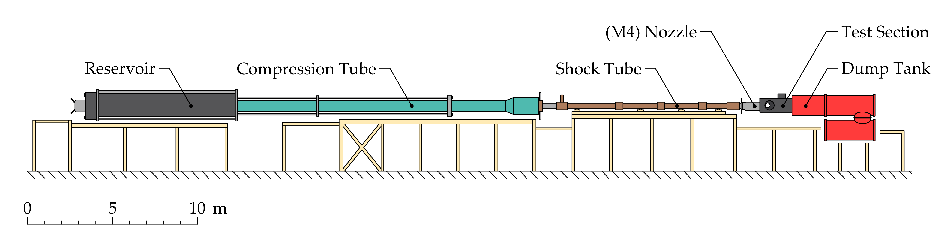
\includegraphics[trim = 0mm 0mm 0mm 0mm, clip, width=0.9\columnwidth]{Figures/T4_Shock_Tunnel_Luke_D_2013.eps}
	\caption{A generic overview of the T4 Stalker Tube. Extracted from ~\cite{Doherty:PhD_Thesis_Scram_M10}.}
	\label{fig:T4_Overview}	
\end{figure}


%%%%%%%%%%%%%%%%%%%%%%%%%%%%%%%%%%%%%%%%%%%%%%%%%%%%%%%%%%%%%%%%%%%%%%%%%%%%%
\section{Experimental Model}
	\label{sec:ModelDescription}

% KDB: I just rearanged this whole paragragh	
Figure ~\ref{fig:Vortex_Sketches} shows the simplified geometry consisting of a flat plate and a normal fin at an angle of attack used to generate the scramjet-inlet like vortices.
The resulting flowfield, with the freestream velocity moving in the positive x direction, generates a vortex through shock-viscous interactions similar to the vortices generated by non-axisymmetric scramjet inlets~\cite{Llobet_PlumeElongation,AFMCpaper2014}.


% A simplified inlet geometry consisting of a flat plate with a normal fin at an angle of attack is used to generate scramjet-inlet-like vortices.
% This geometry and the flowfield it generates are depicted in Fig.~\ref{fig:Vortex_Sketches}.
% The vortex is generated through shock-viscous interactions, similarly to the vortices generated by non-axisymmetric scramjet inlets~\cite{Llobet_PlumeElongation,AFMCpaper2014}.


\begin{figure}[h]
\center
	\subfloat[Vortex formation and fuel plume]{
	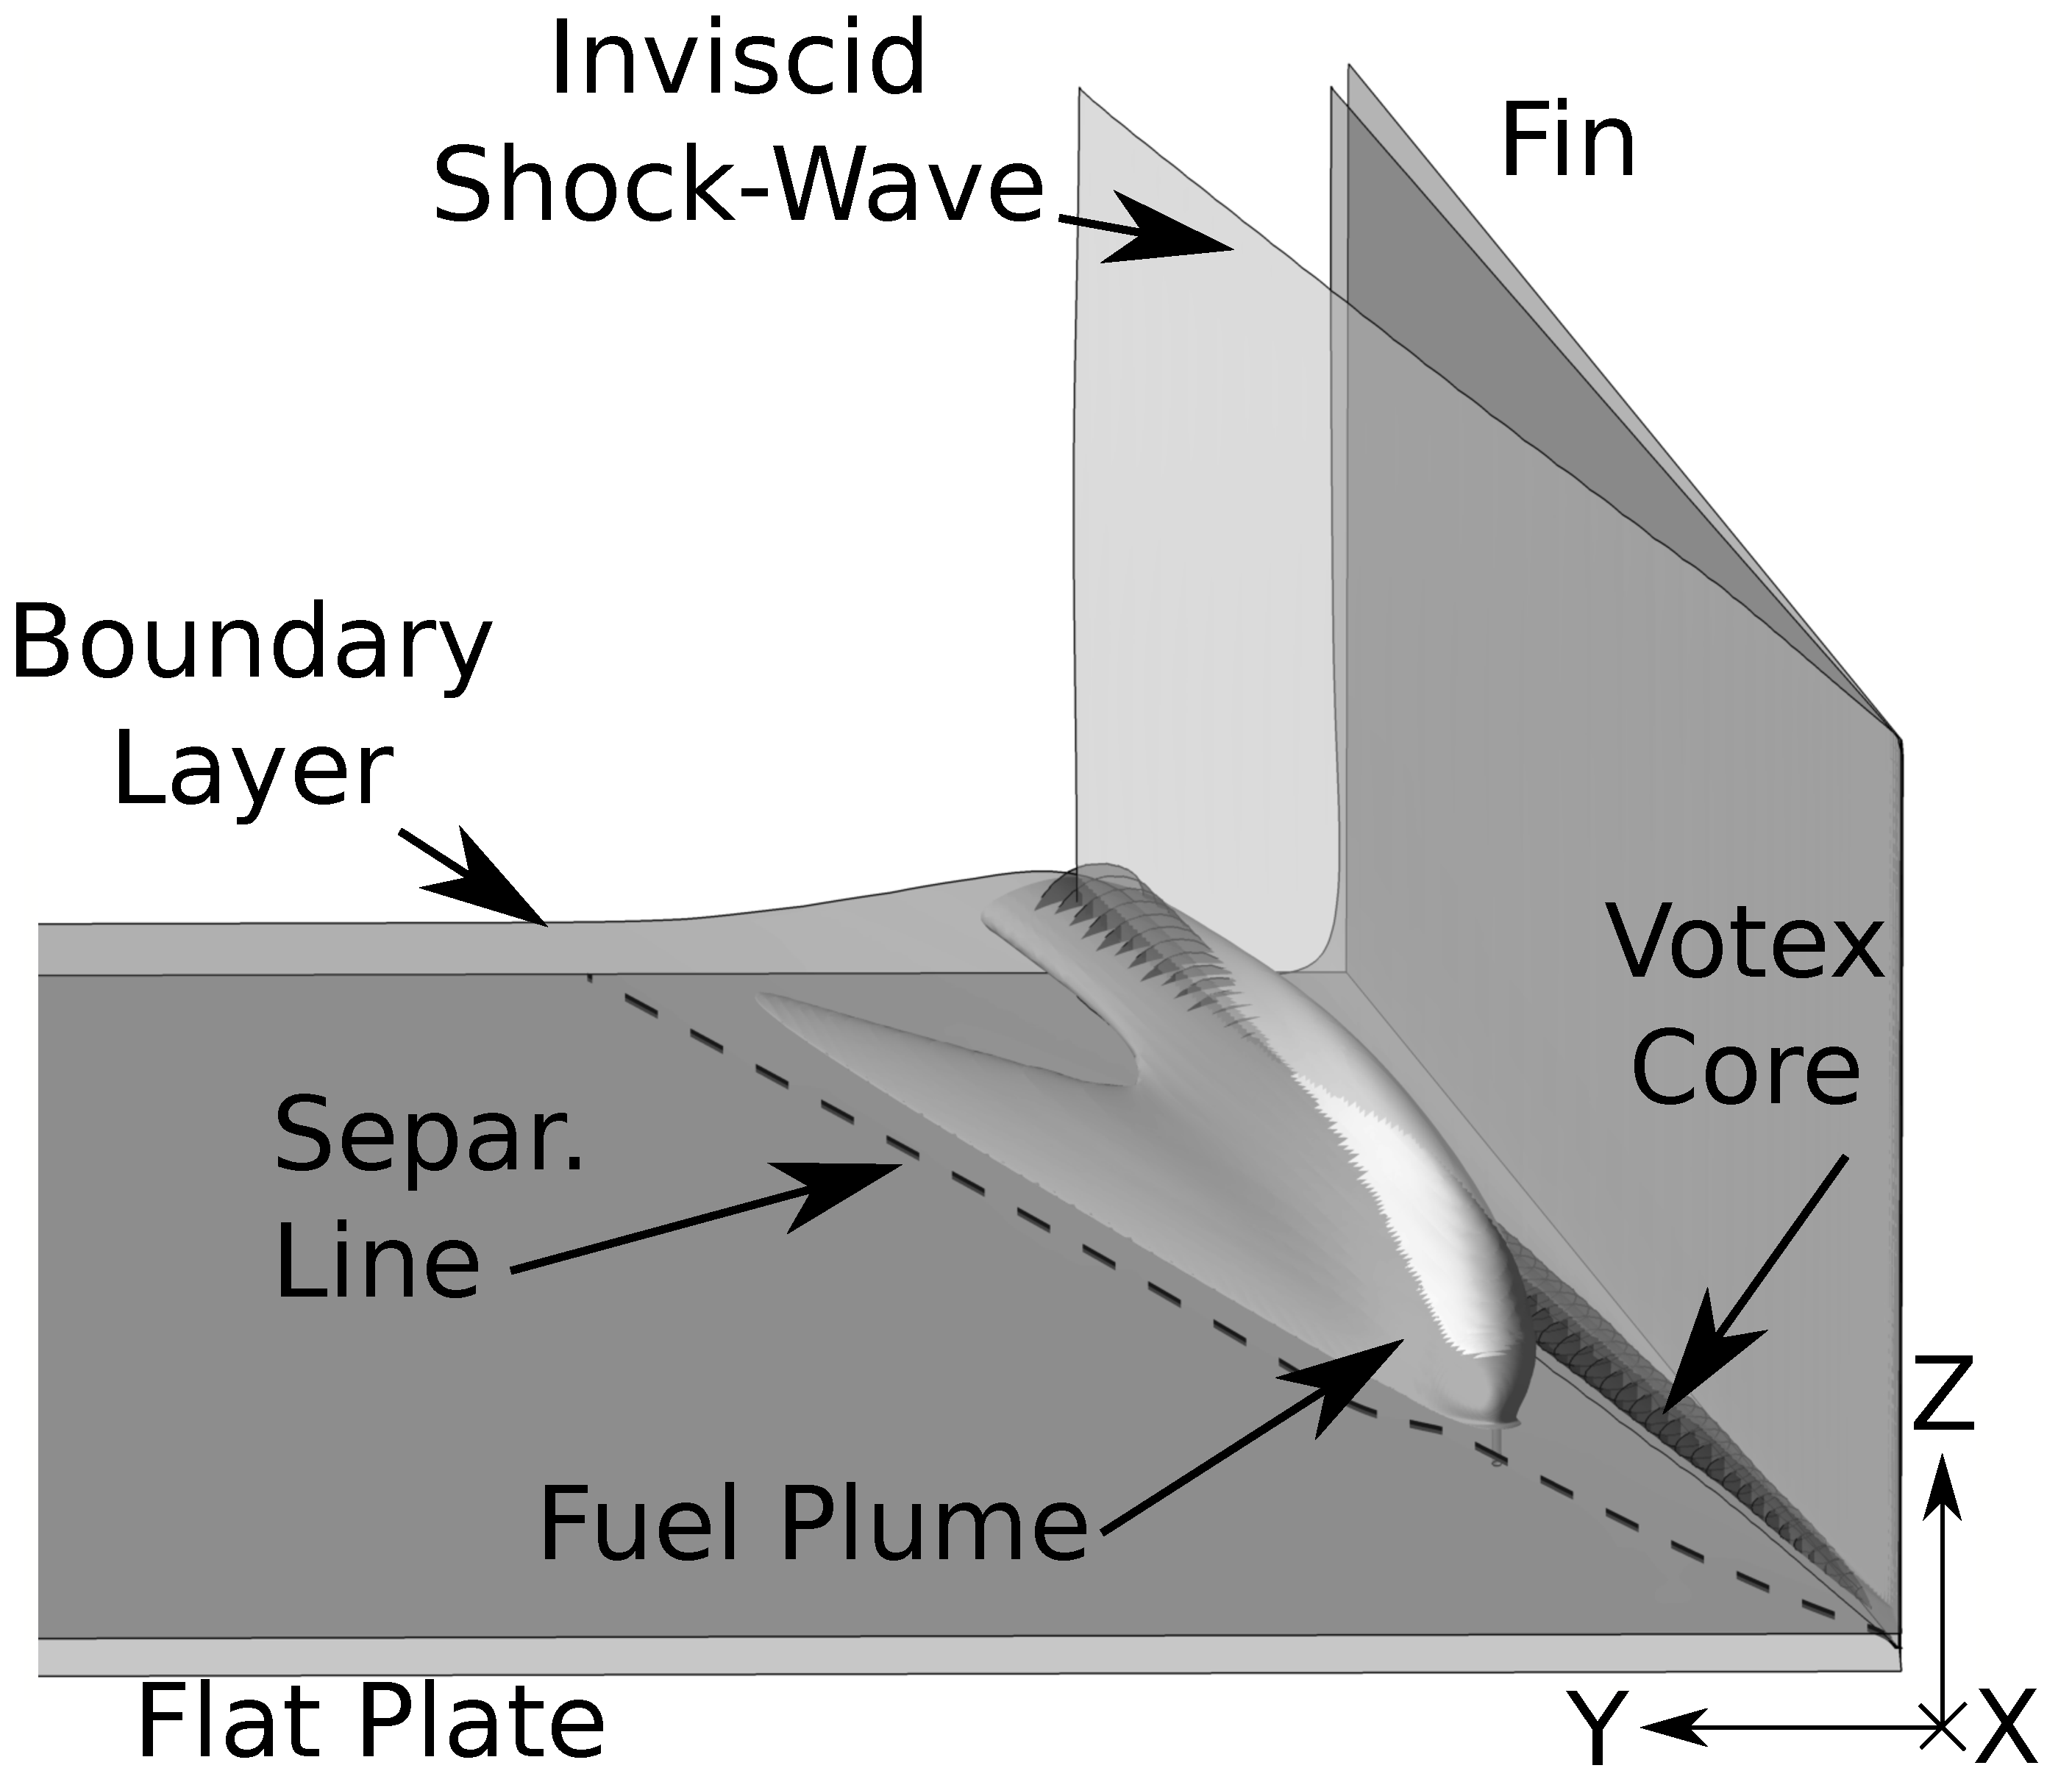
\includegraphics[trim = 0mm 0mm 0mm 0mm, clip, width=0.45\columnwidth]{Figures/Flow_features_V3_B&W.pdf}
	\label{fig:InvShock_BL_Plume}
	}
	\subfloat[Vortex flowfield structure. $\delta$ and contours from  $\alpha_{fin} = 10$ case. Discontinuous lines are adapted from Alvi and Settles~\cite{Alvi}.]{
	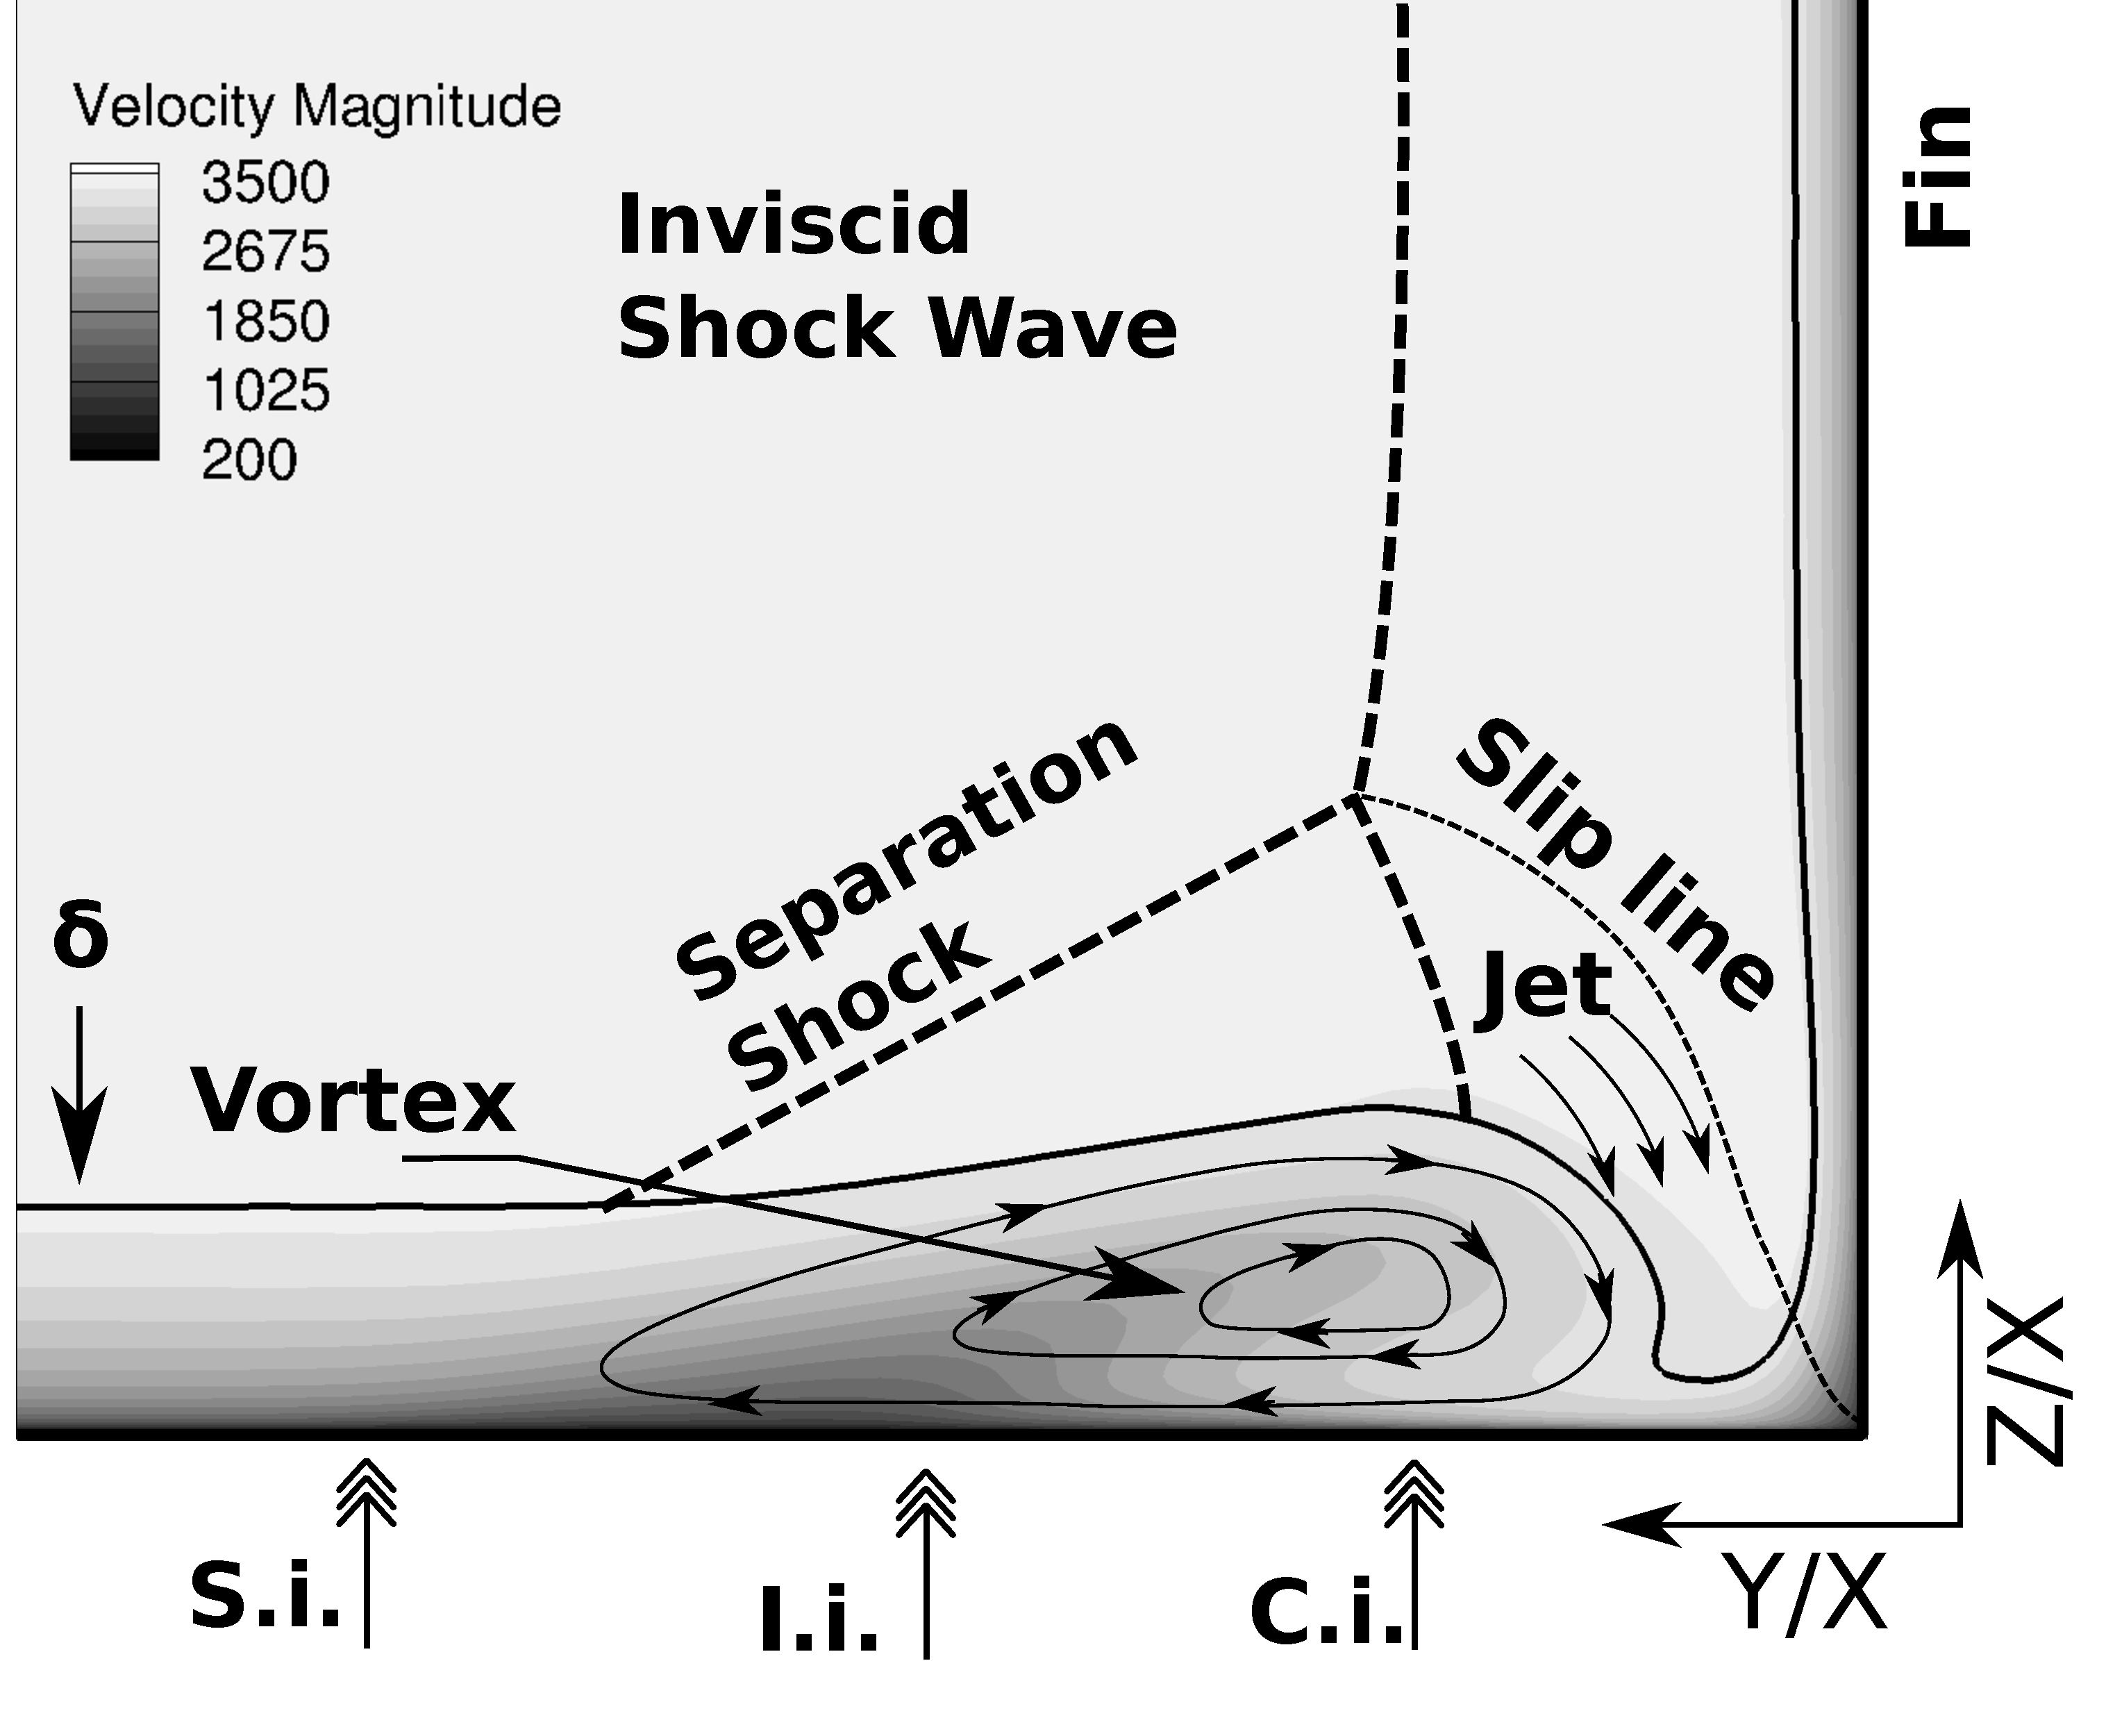
\includegraphics[trim = 2mm 0mm 0mm 2mm, clip, width=0.45\columnwidth]{Figures/AlviSettles_FlowStructure_V5.pdf}
	\label{fig:Alvi_Sketch}
	}
\caption{Test geometry and vortex flowfield structure depiction. Extracted from~\cite{JSASS_paper}}  
\label{fig:Vortex_Sketches}	
\end{figure}


% KDB: Temp formatting to make it more readable.
\hfill\newline


% KDB: As the injector was modified, I don't think you can say equivalent here.
Shown in Fig.~\ref{fig:ModelPics}, the geometry used in the experimental testing is similar to the one used in previous numerical studies~\cite{SpacePlanes_paper2015,AFMCpaper2014,JSASS_paper,Llobet_PlumeElongation}.
% and is depicted in Fig.~\ref{fig:ModelPics}.
For the experimental testing the fin angle was set at \ang{10}.
This angle was chosen due to the relative strength of the vortex generated being representative of the vortices present in previously tested engines~\cite{AFMCpaper2014,SpacePlanes_paper2015}.

% strong vortex withing an intensity representative of that of vortices present in real scramjet inlets~\cite{AFMCpaper2014,SpacePlanes_paper2015}.


%
\begin{figure}[!h]
\center
\subfloat[Model picture.]{
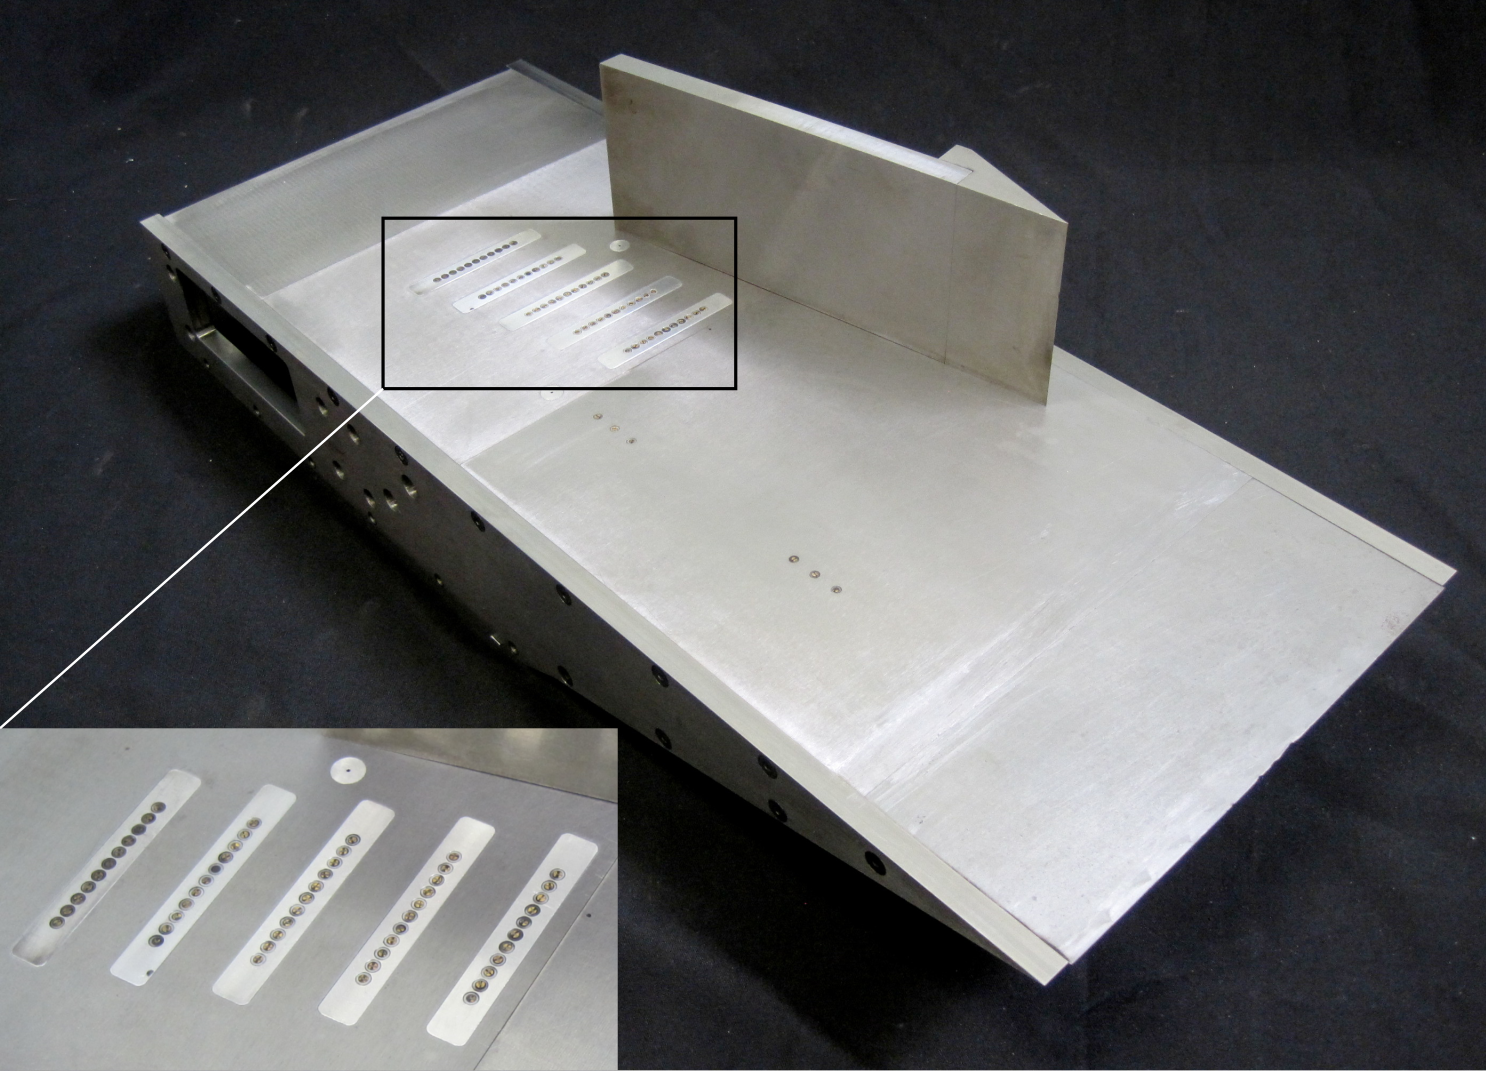
\includegraphics[width=0.50\columnwidth]{Figures/Model_and_zoom.png}
\label{fig:ModelPicture}
}
\subfloat[Detail of gauges distribution location.]{
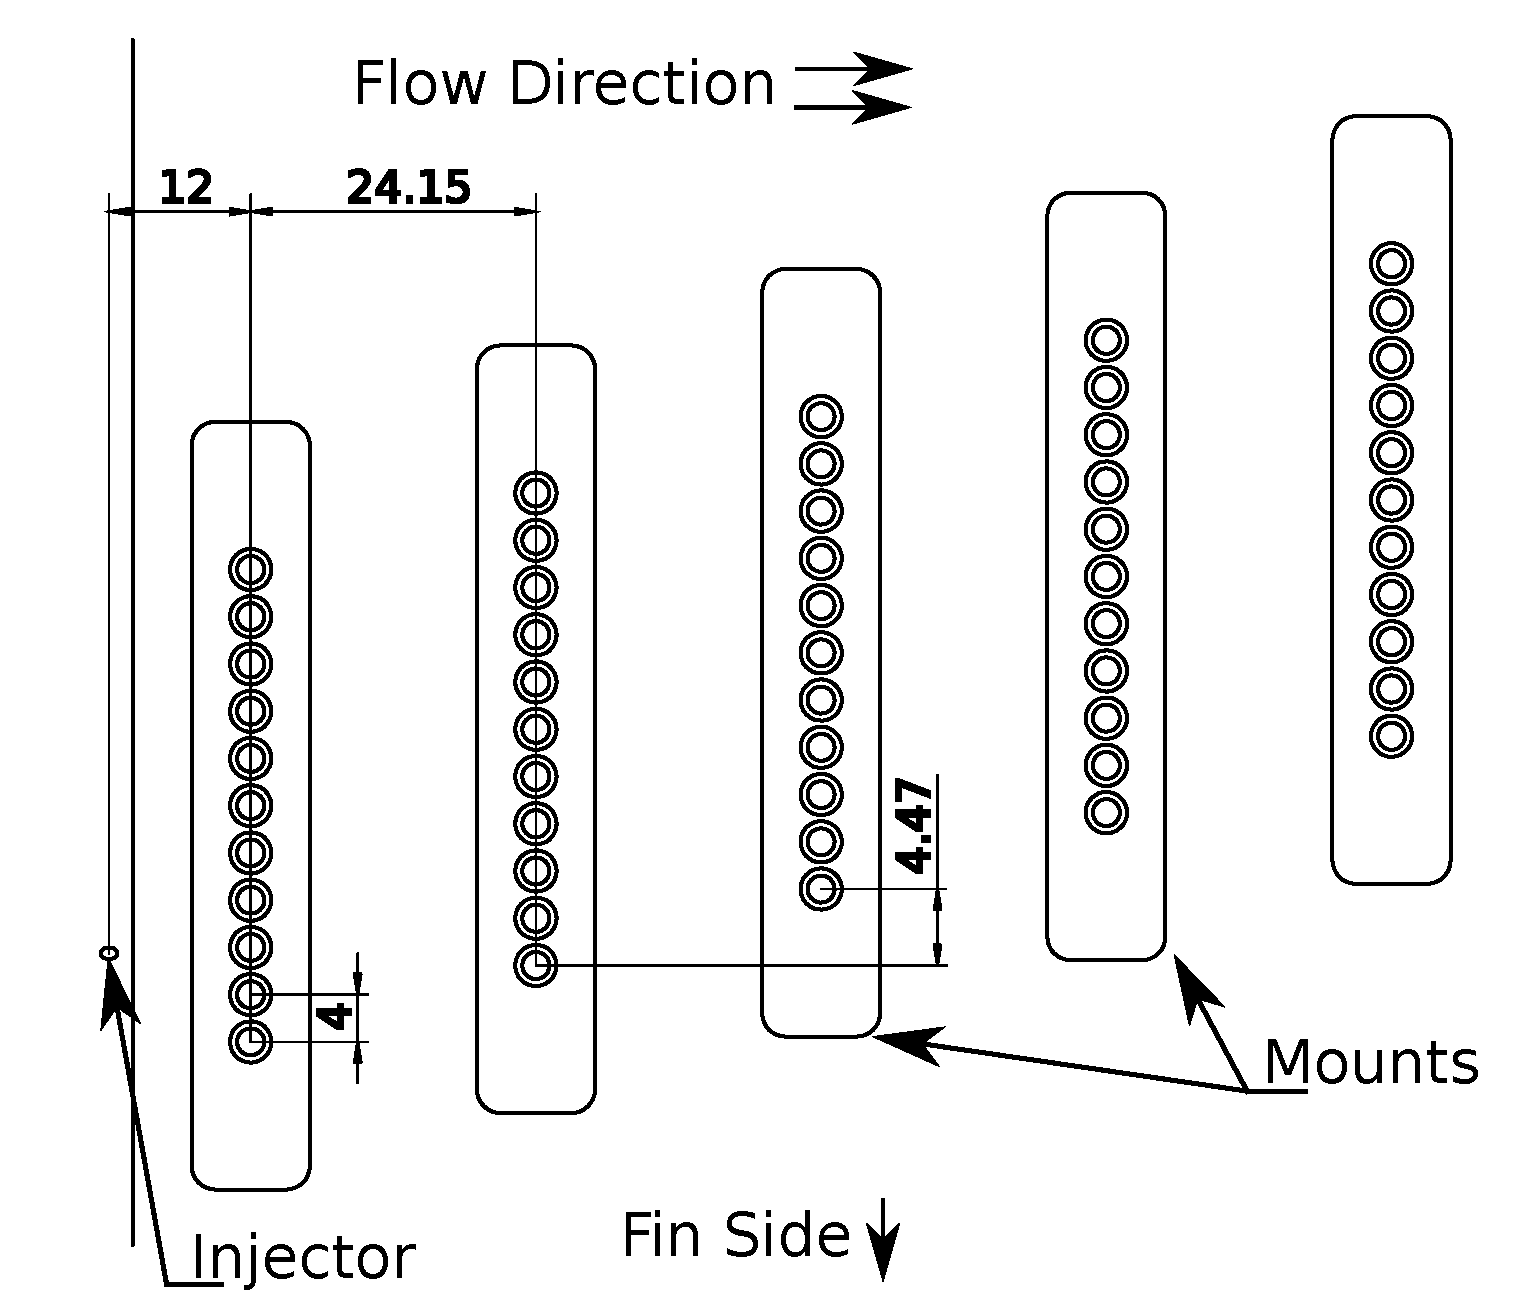
\includegraphics[width=0.40\columnwidth]{Figures/Mounts_Drawing.pdf}
\label{fig:GaugesonModel}
}
\caption{Experimental model in its two configurations.}
\label{fig:ModelPics}
\end{figure} 


The width of the model/plate is $\SI{220}{\milli\meter}$ and was selected to reduce the potential of any three-dimensional effects contaminating the sensor field.
% to avoid any influence of the side-wall 3D effects in the measurement region.
% KDB: 3 sig figs should be fine for this.
% KDB: Probably need to ref the studies again here with the way I've structured it.
The length of flat plate upstream of the fin leading edge was limited to $\SI{156}{\milli\meter}$ due to the potential interference with the tunnel nozzle walls.
The location of the fin and injector were adapted for the experimental testing, when compared to the previous numerical configuration, to accommodate the optical constraints of the T4 test section.
% KDB: Please verify it's diameter for the injector
The $\SI{1}{\milli\meter}$ diameter injector was located $\SI{126}{\milli\meter}$ downstream of the fin leading edge at a $\SI{45}{\deg}$ angle relative to the freestream flow.
% KDB: This needs a simple diagram. I think a top down wireframe with an arrow drawn for the translation would suffice. Nothing crazy.
% KDB: I think you need to define the range it could translate as well in here and probably the resulting Y/X boundary layer heights from the wall. Or something equivalent.
Shown in Fig.~\ref{fig:GaugesonModel}, the fin can be translated in the model Y axis
which allows for different vortex injection locations to be examined. 

% The fin can be translated in the model Y axis to allow for different fin-to-injector distance ratios to be tested.
% Shown in Fig.~\ref{fig:GaugesonModel}, by translating the fin, this allows for different injection locations in the vortex to be examined.


The Thin-Film Heat-transfer Gauges (TFHG) in the model were arranged in five parallel lines as shown in the subset of Fig.\ref{fig:ModelPicture}.
% Heat transfer measurements were obtained along five lines perpendicular to the axial direction.
Each of the gauge lines contains 11 TFHGs that were manufactured at the Centre for Hypersonics. % instrumentation laboratory.
% Data on each line is acquired using eleven thin film heat transfer gauges.
% The thin films used in this experimental campaign were manufactured at the Centre for Hypersonics instrumentation laboratory.
These gauges are made using an $\approx$\SI{20}{\nano\meter} nickel resistive strip element that is sputtered onto an optically smooth quartz substrate.
Shielded with a layer of $SiO_2$, the gauges are individually calibrated after manufacturing ~\cite{Wise_Thesis}.
Once integrated into the experimental model, the heat flux can be calculated using the integrated measured change in the TFHG voltage from a constant current circuit.
% KDB: I feel this needs a linking sentence but I don't really know how at the moment.
This calculation is shown in Eq.~\ref{eq:TFHG_Heat}, from~\cite{Wise_Thesis,Schultz_Book}, where $\rho c k_T$ is the properties of the substrate and $\alpha_R$ is the resistance-independent calibrated TFHG sensitivity.


% KDB: I don't think you need to justify why we use Nickel and quartz. Not the point of your paper.

% The metallic film is a \SI{20}{\nano\meter} Nickel strip.
% The film is sputtered onto an optically smooth quartz substrate~\cite{Wise_Thesis}.
% Nickel was chosen for its high temperature coefficient.
% The properties of quartz vary very little with temperature, making it a good material for the substrate.
% In addition, these gauges are shielded with a layer of $SiO_2$, reducing the wear of the film and avoiding possible short-circuits through an ionized flow~\cite{Wise_Thesis}.
% The sensitivity of the gauges is calculated at the end of the manufacture process.
% The heat flux to the wall can be calculated using Eq.~\ref{eq:TFHG_Heat}, from~\cite{Wise_Thesis,Schultz_Book}, where $\rho c k_T$ are the properties of the substrate, and $\alpha_R$ is the TFHG sensitivity.


\begin{equation}
\dot{q}_n = \frac{\sqrt{\rho c k_T}}{\sqrt{\pi}\alpha_R V_0}\sum^n_{i=1}\frac{V\left(t_0\right)-V\left(t_{i-1}\right)}{\left(t_n-t_i\right)^{1/2}+\left(t_n-t_{i-1}\right)^{1/2}}
\label{eq:TFHG_Heat} 
\end{equation}



Figure~\ref{fig:GaugesonModel} also shows the TFHG sensor field that was required in order to appropriately resolve the heat-transfer profile across the injection-vortex interaction.
%  the gauges had to be mounted in close proximity.
The centers of the gauges are separated by $\SI{4}{\milli\meter}$ in the Y axis, while the lines are separated by $\SI{24}{\milli\meter}$ in the X axis (or freestream direction).
Moreover, the gauge lines have a \SI{4.5}{\milli\meter} offset in the positive Y direction in order to improve the sensor coverage.
The first TFHG line is $\SI{12}{\milli\meter}$ downstream of the injector.


Additionally, the model incorporates six TFHG on the opposite side of the  flat plate to the fin as shown in Fig.~\ref{fig:ModelPicture}.
These gauges are used to measure and identify the state of the boundary layer in the vicinity of the fin leading edge and injection location.
These gauges are grouped in two sets of three $\SI{10}{\milli\meter}$ apart with the 
the first set starting at $\SI{143}{\milli\meter}$ from the flat plate leading edge.
This first group is centered at the same axial location as the fin leading edge in order to determine if the BL was laminar before the start of the vortex.
%  and centered at the same axial location as the fin leading edge.
% The central gauge is located at the same axial distance from the flat plate leading edge as the fin leading edge.
The second set of gauges starts $\SI{249}{\milli\meter}$ downstream of the flat plate leading edge and is located just upstream of the injector.
These gauges are located far enough away from the fin that there is no chance that the resulting shock-wave and vortex could influence the data.
% Therefore, the measurements correspond to the boundary layer unaffected by the vortex.
The boundary layer was found to remain laminar for all test conditions presented in this paper.

Two pressure tabs on the flat plate surface incorporating kulite pressure transducers were used to ascertain the pressure of the nozzle exit conditions.



%%%%%%%%%%%%%%%%%%%%%%%%%%%%%%%%%%%%%%%%%%%%%%%%%%%%%%%%%%%%%%%%%%%%%%%%%%%%%
\subsection{T4 test flow conditions}

The experiments were performed using the T4 Mach 7.6 nozzle at a Mach 8 flight-enthalpy.
The nozzle exit flow conditions are derived from measurements of the shock tube fill pressure $\left(P_{ST}\right)$, shock tube shock-speed $\left(V_{S}\right)$, shock tube temperature $\left(T_{ST}\right)$, and the stagnation region nozzle supply pressure $\left(P_e\right)$.
Shown in Table~\ref{tab:Exper_Flow_Cond} is the calculated nozzle exit values tabulated along with their uncertainties.

% The nozzle exit values are tabulated along with their uncertainties in Table~\ref{tab:Exper_Flow_Cond}.


% KDB: Changing this to 3 sig figs

\begin{table}[!h]
\centering
\caption{Nominal conditions during testing a nozzle exit.}
\label{tab:Exper_Flow_Cond}
\begin{tabular}{rl|rl}
\multicolumn{2}{c|}{Variable} & \multicolumn{2}{c}{Value}\\
\hline
\Gape[0.2cm][0.0cm]{$P_0$} & $[\SI{}{\mega\pascal}]$		& $15.7$ 	& $\pm 4.42\%$ \\
$P_\infty$ 		& $[\SI{}{\kilo\pascal}]$				& $2.29$ 	& $\pm 4.53\%$  \\
$T_\infty$ 		& $[\SI{}{\kelvin}]$						& $237$ 	& $\pm 7.37\%$ \\
$\rho_\infty$	& $[\SI{}{\kilo\gram\per\cubic\meter}]$	& $0.0335$ 	& $\pm 6.97\%$ \\
$u_\infty$ 		& $[\SI{}{\meter\per\second}]$			& $2340$	& $\pm 2.98\%$ \\
$M_\infty$ 		& $[-]$									& $7.57$ 	& $\pm 0.70\%$ \\           
$H_0$ 			& $[\SI{}{\mega\joule\per\kilo\gram}]$	& $2.73$ 	& $\pm 7.10\%$ \\          
\hline
\end{tabular}
\end{table}


The nozzle exit conditions shown in Table~\ref{tab:Exper_Flow_Cond} are calculated using the in-house code NENZFr from the University of Queensland~\cite{nenzfr_manual}.
NENZFr is a wrapper that integrates an ESTCj(\textbf{[ref]}) shock-tube simulation into a space-marched thermal and chemical non-equilibrium Eilmer3 CFD simulation of the nozzle.
Eilmer3 is a collection of programs simulating 2-D/3-D thermal and chemical non-equilibrium transient Navier-Stokes that is also developed at the University of  Queensland~\cite{Eilmer_TheoryBook,Eilmer3UserGuide}.


The axisymmetric grid used for the space-marched Eilmer3 simulation is constructed by inscribing a uniform structured grid between a Bezier curve defining the nozzle wall and the nozzle centerline.
The mesh employed in this study consisted of 600 by 40 elements in the axial and radial directions respectively.
The chemical composition of the gas is calculated using finite-rate reactions with a five species air model: $N_2$, $O_2$, $NO$, $N$ and $O$.
The thermodynamic properties are obtained using NASA CEA2~\cite{CEA2,Eilmer_TheoryBook}.


% KDB: Luke uses a 100% for the transiiton location. His condition comes out to about -0.63 which with an assumed 1% for the kulites this should be true.
Moreover, to improve the accuracy of the nozzle exit conditions an iterative convergence was applied to the transition location in the nozzle.
The baseline predictive value was iterated upon until a satisfactory convergence was found with the experimentally measured static pressure on the plate.
The uncertainty of this measurement is lower than the resultant sensitivity from the nozzle transition location, and thus is considered a truth value target for the iterative convergence\cite{Doherty:PhD_Thesis_Scram_M10}.



% KDB: Remove all this once you're happy with my edits. I changed a lot... :/


% the transition onset location on the T4 nozzle wall surface is required.
% The length at which transition takes place is unknown.
% For this reason, a parametric study was performed, varying this parameter until the static pressure at the nozzle exit closely matched the experimental pressure measured on the flat plate.

% The equations are solved using an upwind scheme.

% The code has been specifically tailored to accurately the flow in reflected shock tunnels and expansion shock tunnels.

% The nozzle exit values in Table~\ref{tab:Exper_Flow_Cond} are calculated using NENZFr.
% NENZFr~\cite{nenzfr_manual} is a set of scripts that coordinate a space-marched nozzle simulation in the CFD code Eilmer3, developed at University of Queensland.
% Eilmer3 is a collection of programs simulating 2-D/3-D Navier-Stokes transient compressible flow~\cite{Eilmer_TheoryBook,Eilmer3UserGuide}.
% It is specialized in solving accurately the flow in reflected shock tunnels and expansion shock tunnels.
% The equations are solved using an upwind scheme.
% Moreover, it calculates thermochemistry and finite-rate chemistry processes within the flowfield. 
 


%%%%%%%%%%%%%%%%%%%%%%%%%%%%%%%%%%%%%%%%%%%%%%%%%%%%%%%%%%%%%%%%%%%%%%%%%%%%%
\section{Test cases}

Two fin locations in the model Y axis were examined as a part of the experimental campaign.
Both of these locations corresponded to different relative injection locations in the vortex in order to verify how the effusing fluid influenced the resulting flowfield.
% KDB: I think you need to show this. Remove if you don't want.
The approximate locations relative to the induced vortex are shown on Fig. \ref{fig:Alvi_Sketch}.
These locations were measured as the perpendicular distance to the fin in the model Y axis  non-dimensionalized by the jet diameter.
% KDB: Please make sure I didn't get the distance wrong. Also, I "nondimensionalized" by jet diameter which still keeps everything the same
% as the minimum spanwise distance between the fin and the injector center with respect to the injector are used.
The corresponding fin-to-injector distance ratios tested were $26.2$ and $35.2$, and are named the Upper Fin (UF), and Lower Fin (LF) test cases respectively.


Hydrogen was used as the injection fluid for this campaign and was tested at two different plenum pressures at both of the UF and LF locations.
The two pressures tested were $P_{inj}=\SI{1300}{\kilo\pascal}$ and $P_{inj}=\SI{430}{\kilo\pascal}$ and are named the High Injection (HI) and Low Injection (LI) cases respectively.
These two pressures produce injection-to-freestream momentum ratios of $5.24$, and $1.73$ with a Ludwieg tube used in order to maintain a constant total plenum pressure.
%  during the facility test time.
% The total pressure inside the injector plenum  maintained constant during the test time using a Ludwieg tube.
The case of No Injection (NI) was used to obtain the baseline undisturbed vortex heat flux data.


All of these parameters were combined to produce six different test cases as summarized in Table~\ref{tab:T4_Test_Cases}.
	

% Hydrogen fuel is injected through a \SI{1}{\milli\meter} diameter injector inclined \ang{45} in the axial direction.


\begin{table}[!h]
\centering
\caption{Combination of injection pressure and fin position for the different test cases.}
\label{tab:T4_Test_Cases}
\begin{tabular}{lc|c|c}
	$\#$ & Naming  & Injection Pressure & \specialcell{Fin-to-injector\\distance ratio}\\
\hline
\Gape[0.2cm][0.0cm]{1} & NI-UF & - (-) &  $26.2$\\
2 & NI-LF & - (-) &  $35.2$ \\
3 & HI-UF & $\SI{1300}{\kilo\pascal}$ $\pm\SI{3.1}{\percent}$ &  $26.2$ \\
4 & LI-UF & $\SI{430}{\kilo\pascal}$ $\pm\SI{2.8}{\percent}$ &  $26.2$ \\
5 &	HI-LF &  $\SI{1300}{\kilo\pascal}$ $\pm\SI{3.1}{\percent}$ &  $35.2$ \\
6 & LI-LF & $\SI{430}{\kilo\pascal}$ $\pm\SI{2.8}{\percent}$ &  $35.2$ \\

\hline
\end{tabular}
\end{table}


%%%%%%%%%%%%%%%%%%%%%%%%%%%%%%%%%%%%%%%%%%%%%%%%%%%%%%%%%%%%%%%%%%%%%%%%%%%%%
\section{CFD reference results}
\label{sec:CFDReferenceRes}

The data obtained in the experiments is complemented with numerical simulations to enhance the understanding of the results and assess the validity of the numerical methodology.
The numerical domain used spans from $\SI{10}{\milli\meter}$ upstream to $\SI{300}{\milli\meter}$ downstream of the fin leading edge and $\SI{200}{\milli\meter}$ centered around the injector centroid in the spanwise direction.
The boundary layer development over the first $\SI{146}{\milli\meter}$ of the flat plate upstream of the fin leading edge was calculated in a separate quasi two-dimensional simulation with an infinitely sharp leading edge. 
The resulting exit profile from this simulation was input as an infinite plane into the three-dimensional numerical domain described above.
% KDB: Probably want to check my statement on this one mate.
%, and used as the inflow for the main 3-D flow calculations.

% KDB: I'm assuming that this was structured for US3D?

The structured three-dimensional domain contained approximately four million cells and had a minimum spacing around the injector of approximately $\SI{0.05}{\milli\meter}$.
The cell growth from the injector was restricted to $\SI{1}{\milli\meter}$ in the region of uniform flow and was considered a far-field approximation from the vortex-injection interaction.
% Within the injector vicinity, the cells size is approximately $\SI{0.05}{\milli\meter}$, expanding up to $\SI{1}{\milli\meter}$ in the region of uniform flow, far from the vortex-injection interaction.
Inside the numerical domain, the injector was placed at $X=\SI{125}{\milli\meter}$ downstream of the fin leading edge and 26.2 and 35.2 fin-to-injector distances ratios in order to match the experiments.
% KDB: I'm unsure about this grammar usage but just rolling with it for now. 
The walls were modeled as non-slip isothermal with a temperature at $\SI{300}{\kelvin}$ --- the mean for the lab in which the experiments were conducted. 
% The injector in the numerical domain was placed at $X=\SI{125}{\milli\meter}$ downstream of the fin leading edge in order to match the experiments.
% In the spanwise direction, the injector is placed at $Y=\SI{26.2}{\milli\meter}$ from the fin leading edge in the UF case, and $Y=\SI{35.2}{\milli\meter}$ in the LF case.


The inflow conditions used for the simulations are the nominal conditions calculated at the nozzle exit in Table~\ref{tab:Exper_Flow_Cond}.
Using the transition predictions for the T4 tunnel from He and Morgan[\textbf{ref}], the plate was expected to stay fully laminar upstream of the oblique shock and injector.
% KDB: Take this out if you want. I would recommned keeping the He and Morgan reference though
Thus, the pseudo-2D simulations were conducted as fully laminar and no boundary layer parabolic stability transition prediction was used.
% As transition is only anticipated downstream of the oblique shock and injector, the pseudo-2D simulations are performed as fully laminar. 

% The main three-dimensional simulations of the flat plate plus fin are performed with the
The turbulence model used was an SST $k-\omega$ to allow for a more accurate turbulent mixing of the fuel and the production of turbulence in the boundary layer region separated by the fin shock.
In order to accommodate the laminar inflow from the quasi-2D simulation, the 3D domain inflow Turbulent Kinetic Energy (TKE) was set to zero.
% To achieve this, the turbulence parameters are incorporated to the laminar inflow data with a value of zero at the domain inflow.
By setting this value to zero, the laminar nature of the flow upstream of the fin, as seen in the experiments, was able to be replicated for most of the flat plate.
More importantly, using a zero TKE inflow with the SST $k-\omega$, allowed for an appropriate modeling of the viscous turbulence generation in the laminar boundary layer interaction with the fin shock as well as the separations and injection-vortex interaction.
% the combination of the laminar inflow with the SST $k-\omega$ model computation produces an effectively laminar boundary layer interaction with the fin shock, while allowing the generation of turbulence in the separation and injection regions.
This TKE generation can be seen in Fig.~\ref{fig:TurbKinEn_CFD_SliceLow} with the one dimensional extraction slice taken along the line displayed in the figure.
% , as taken from the slice in Fig.~\ref{fig:TurbKinEn_CFD_SliceLow}.
Examining this subset extraction in Fig.~\ref{fig:TurbKinEn_CFD_SliceLow}, the TKE remains almost negligible in the initial part of the domain until a rapid onset just downstream of the injector.
Thanks to the delayed onset of TKE growth, the flow relevant for the region of interest remains laminar until its separation, qualitatively representing the turbulent state of the flow in the experiments.
The good agreement between the numerical and experimental results for the laminar region can be seen in Fig.~\ref{fig:Exp_Num_Q}.
% The good agreement between the numerical and experimental flow conditions in the fully laminar region is depicted in Fig~\ref{fig:Exp_Num_Q}.


\begin{figure}[!h]
\center
\subfloat[Turbulent kinetic energy (TKE) evolution in the numerical case.]{
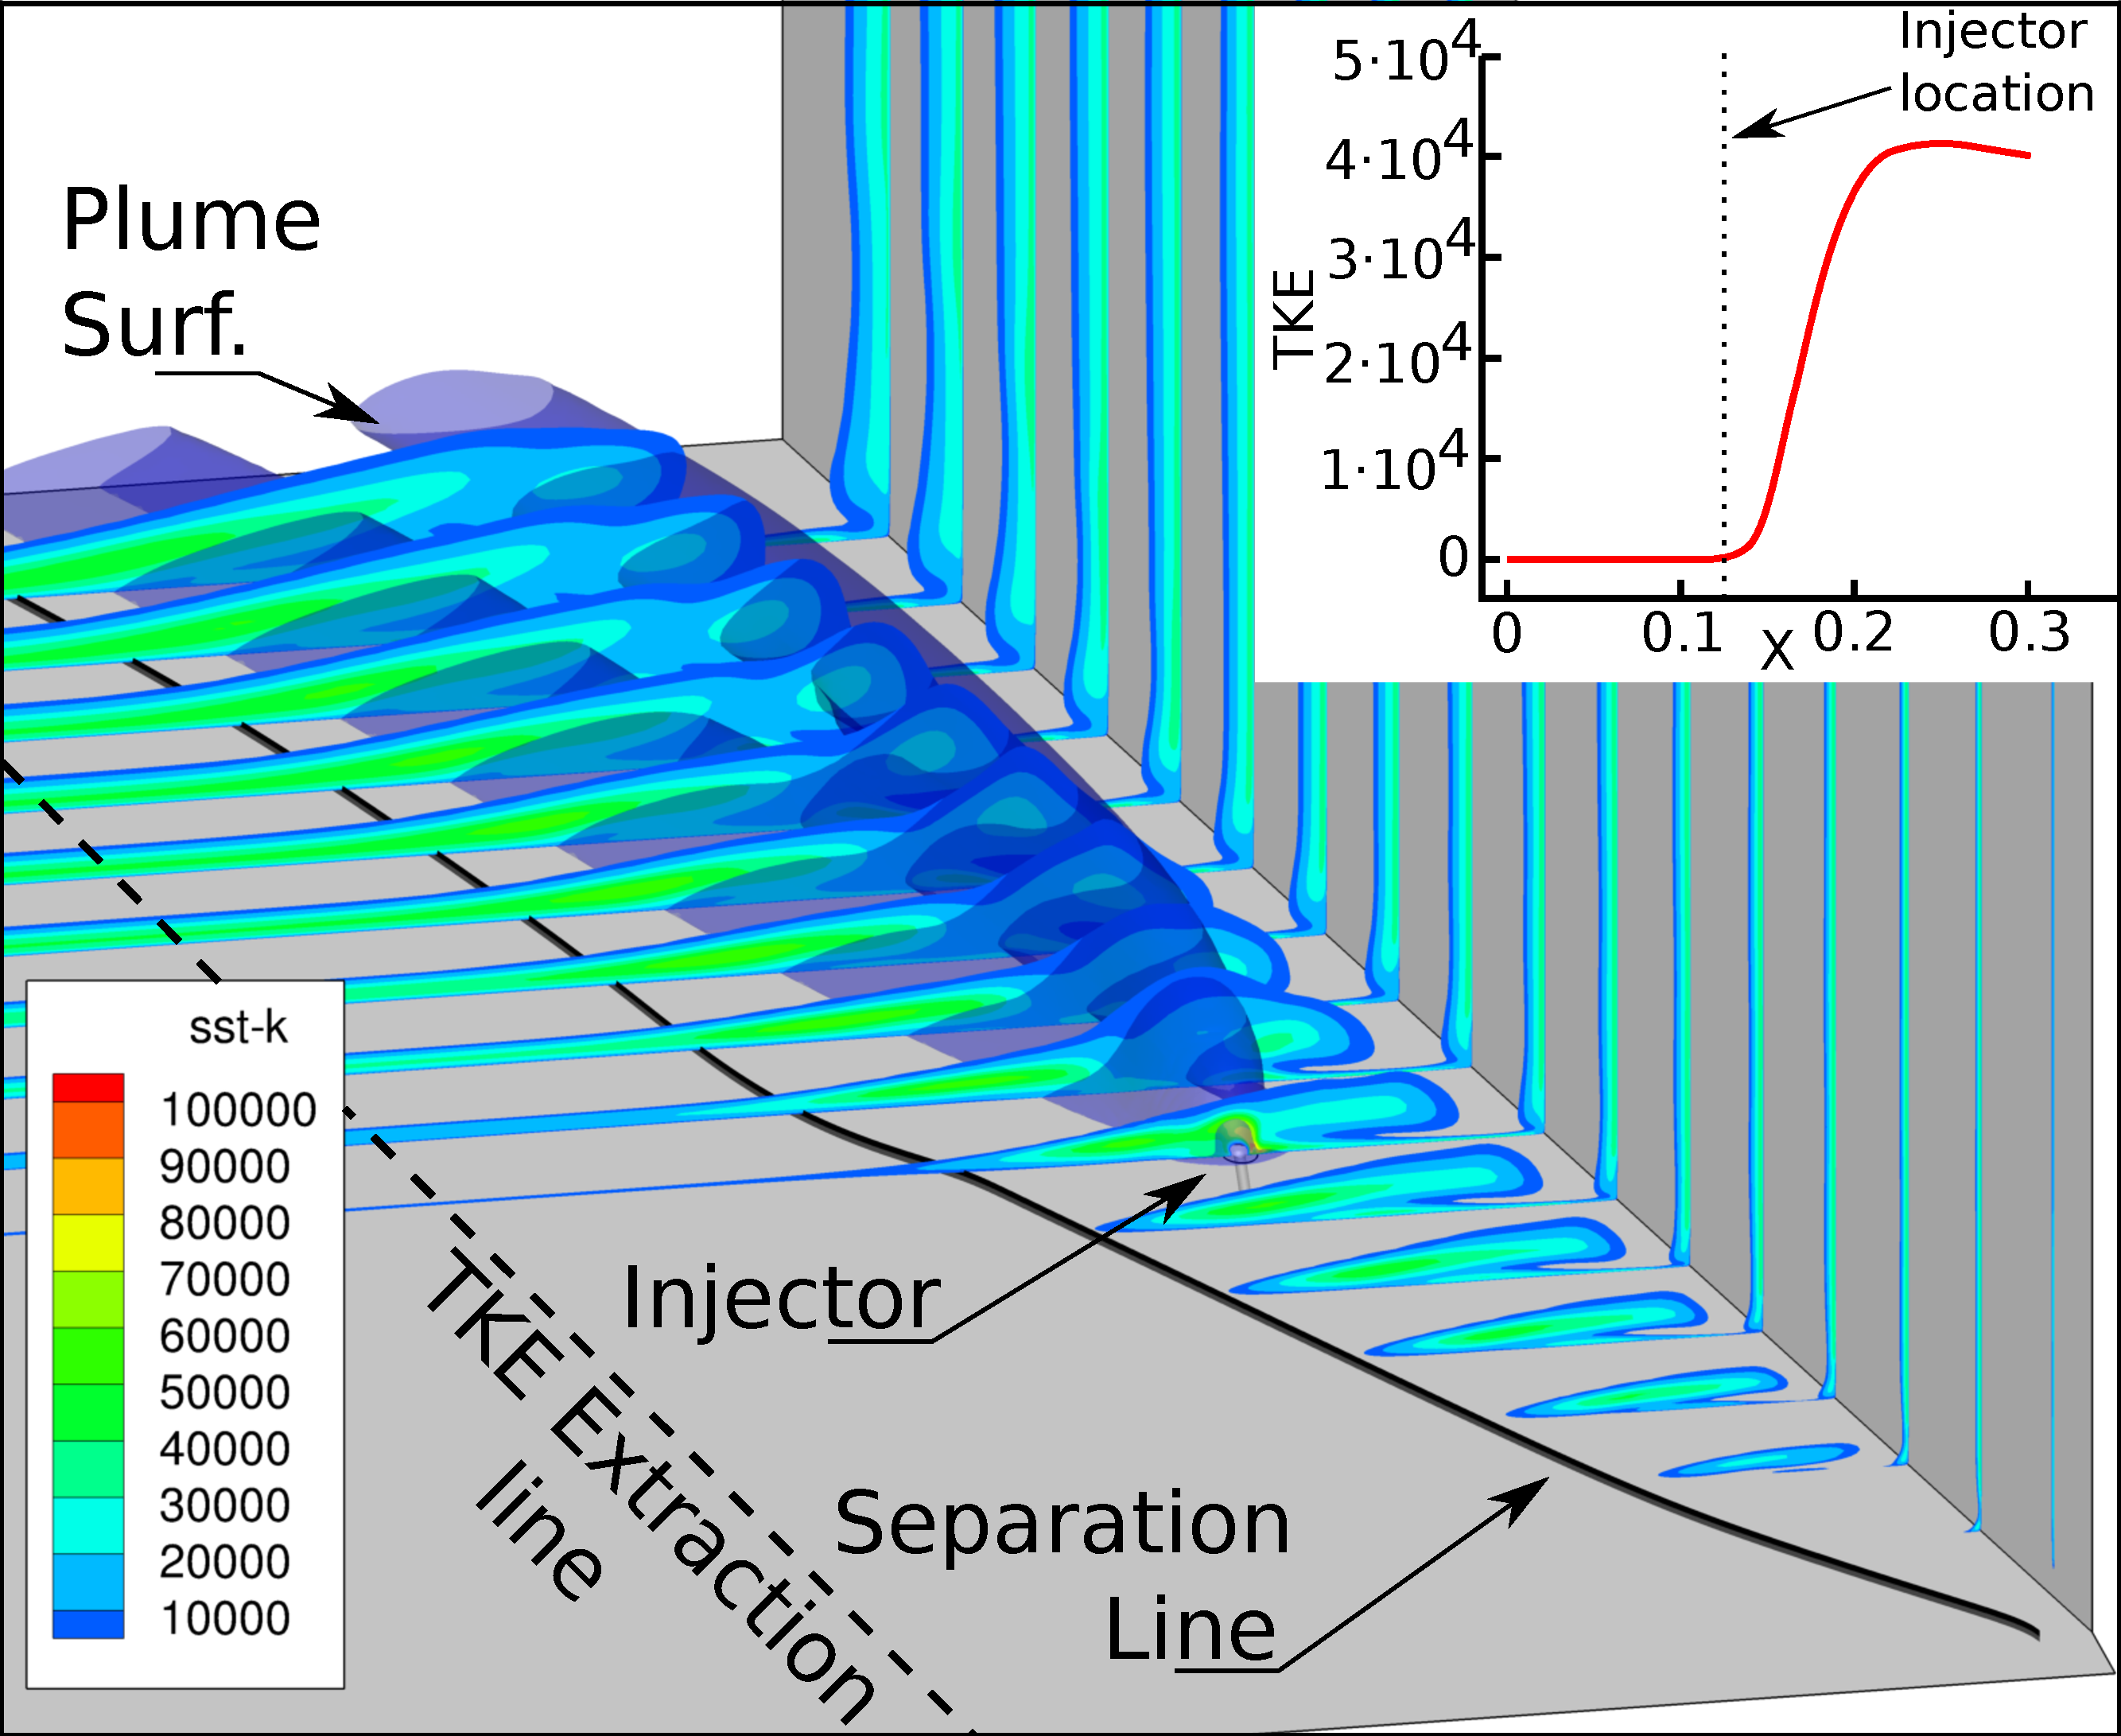
\includegraphics[trim = 0mm 0mm 0mm 0mm, clip, width=0.45\columnwidth]{Figures/TurbKinEnergySlices_csH2Stoich_LowP_LowF_HighInj_fmt_V2.pdf}
\label{fig:TurbKinEn_CFD_SliceLow}
}
\subfloat[Experimental and numerical heat flux on the undisturbed flat plate region.]{
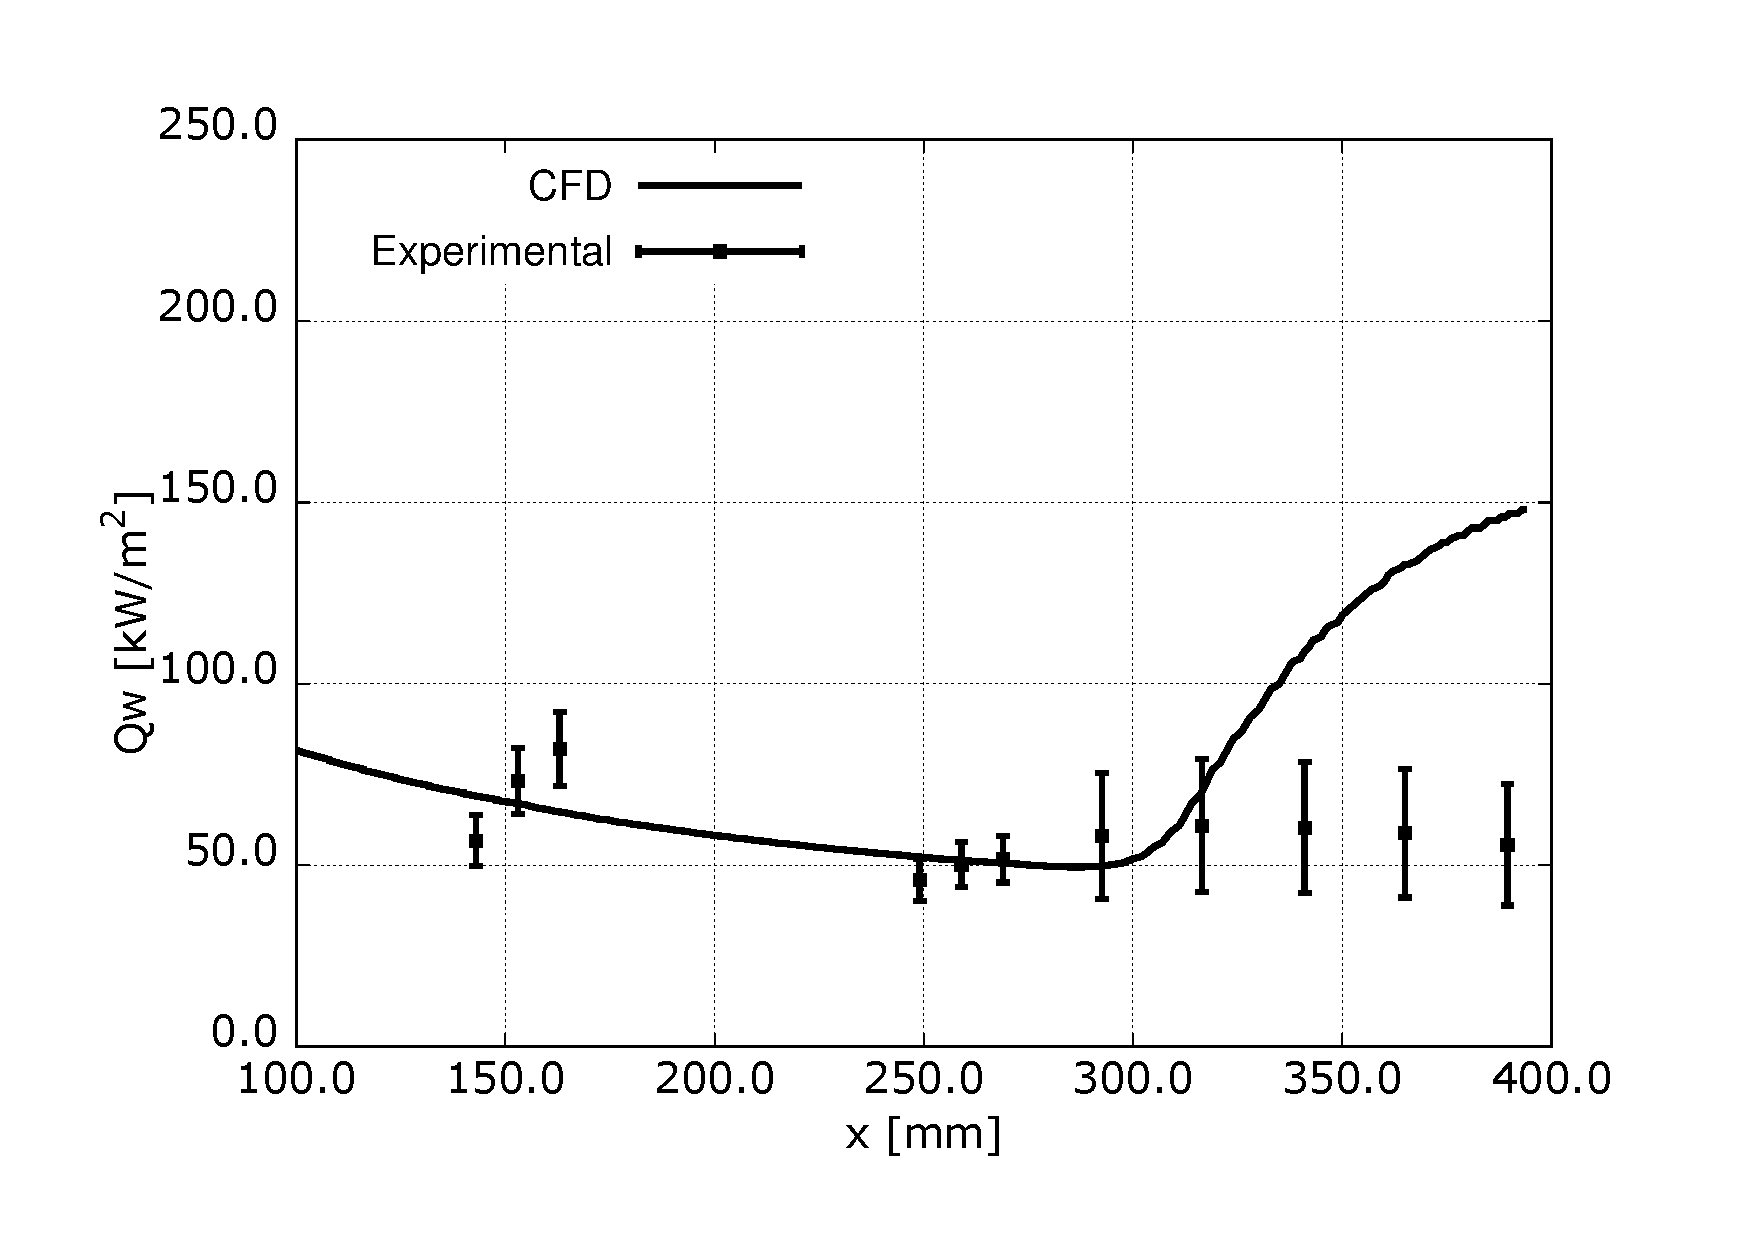
\includegraphics[trim = 0mm 6mm 25mm 18mm, clip, width=0.54\columnwidth]{Figures/GNUP_LP_CFD-EXP_Comparison.pdf}
\label{fig:Exp_Num_Q}
}
\caption{Boundary layer state comparison between the experimental and numerical cases}
\label{fig:Num_Exp_BLcompar}
\end{figure} 



%%%%%%%%%%%%%%%%%%%%%%%%%%%%%%%%%%%%%%%%%%%%%%%%%%%%%%%%%%%%%%%%%%%%%%%%%%%%%
\section{Results}

The experimental and numerical data obtained is presented in this section. The case with no injection is presented first, followed by the study of the vortex-injection cases.

%%%%%%%%%%%%%%%%%%%%
\subsection{Unfueled vortex}

Two tests using the the Upper and Lower fin positions with no injection were performed to identify the effect of the vortex on heat flux, and the ability of the numerical methodology to accurately simulate this flowfield.

The experimental data along the lines formed by the gauges on each mount are presented in Fig.~\ref{fig:LP-NI-UF_LinesPlots} and Fig.~\ref{fig:LP-NI-LF_LinesPlots} for the Upper and Lower fin positions respectively.
%LP_NoI_UF
\begin{figure}[!h]
\center
%\begin{adjustbox}{max width=1.1\columnwidth,center}
\subfloat[Upper fin position.]{
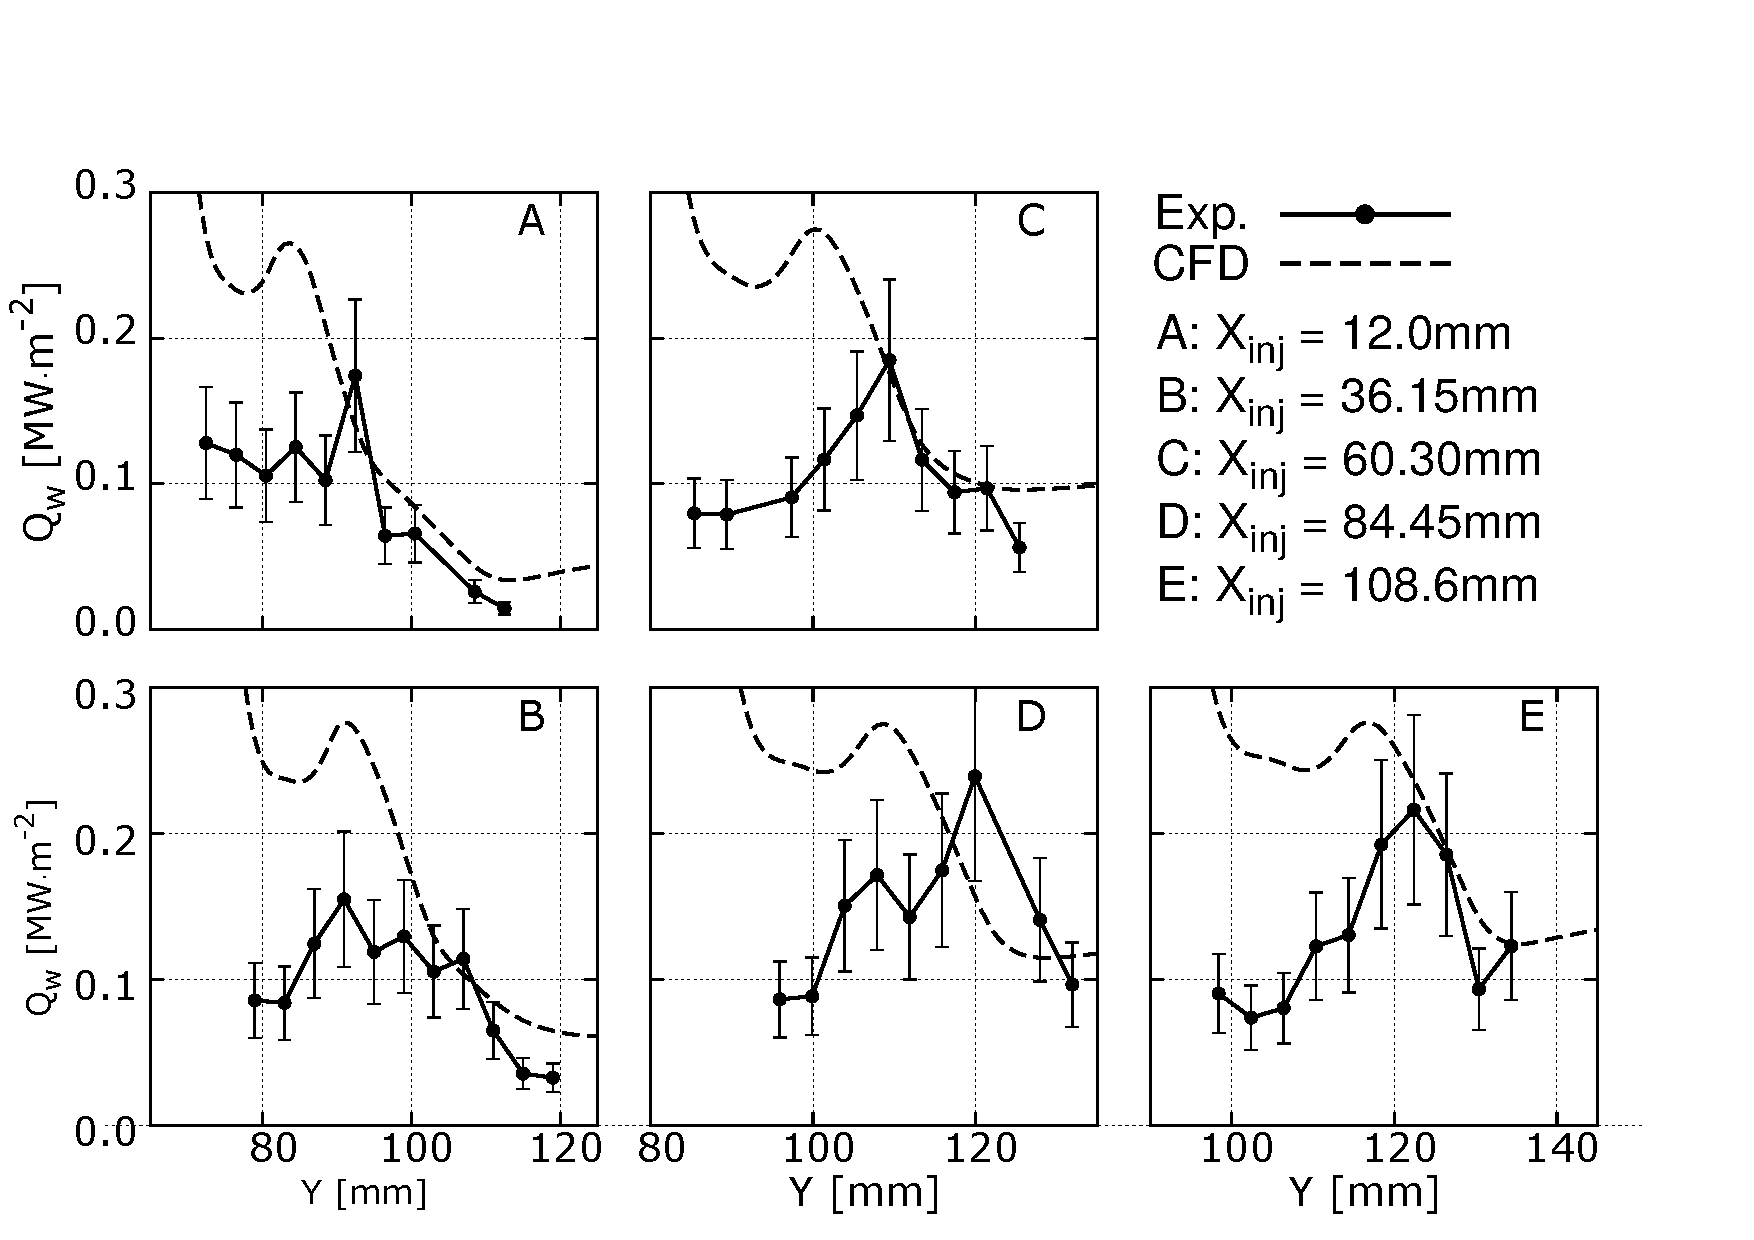
\includegraphics[trim = 0mm 3mm 25mm 25mm, clip, width=0.60\columnwidth,valign=t,fbox]{Figures/Data/LP_NoI_UF/GNUP_CFD_GaugesLines_Multi.pdf}
\label{fig:LP-NI-UF_LinesPlots}
}
%
\\
\subfloat[Lower fin position.]{
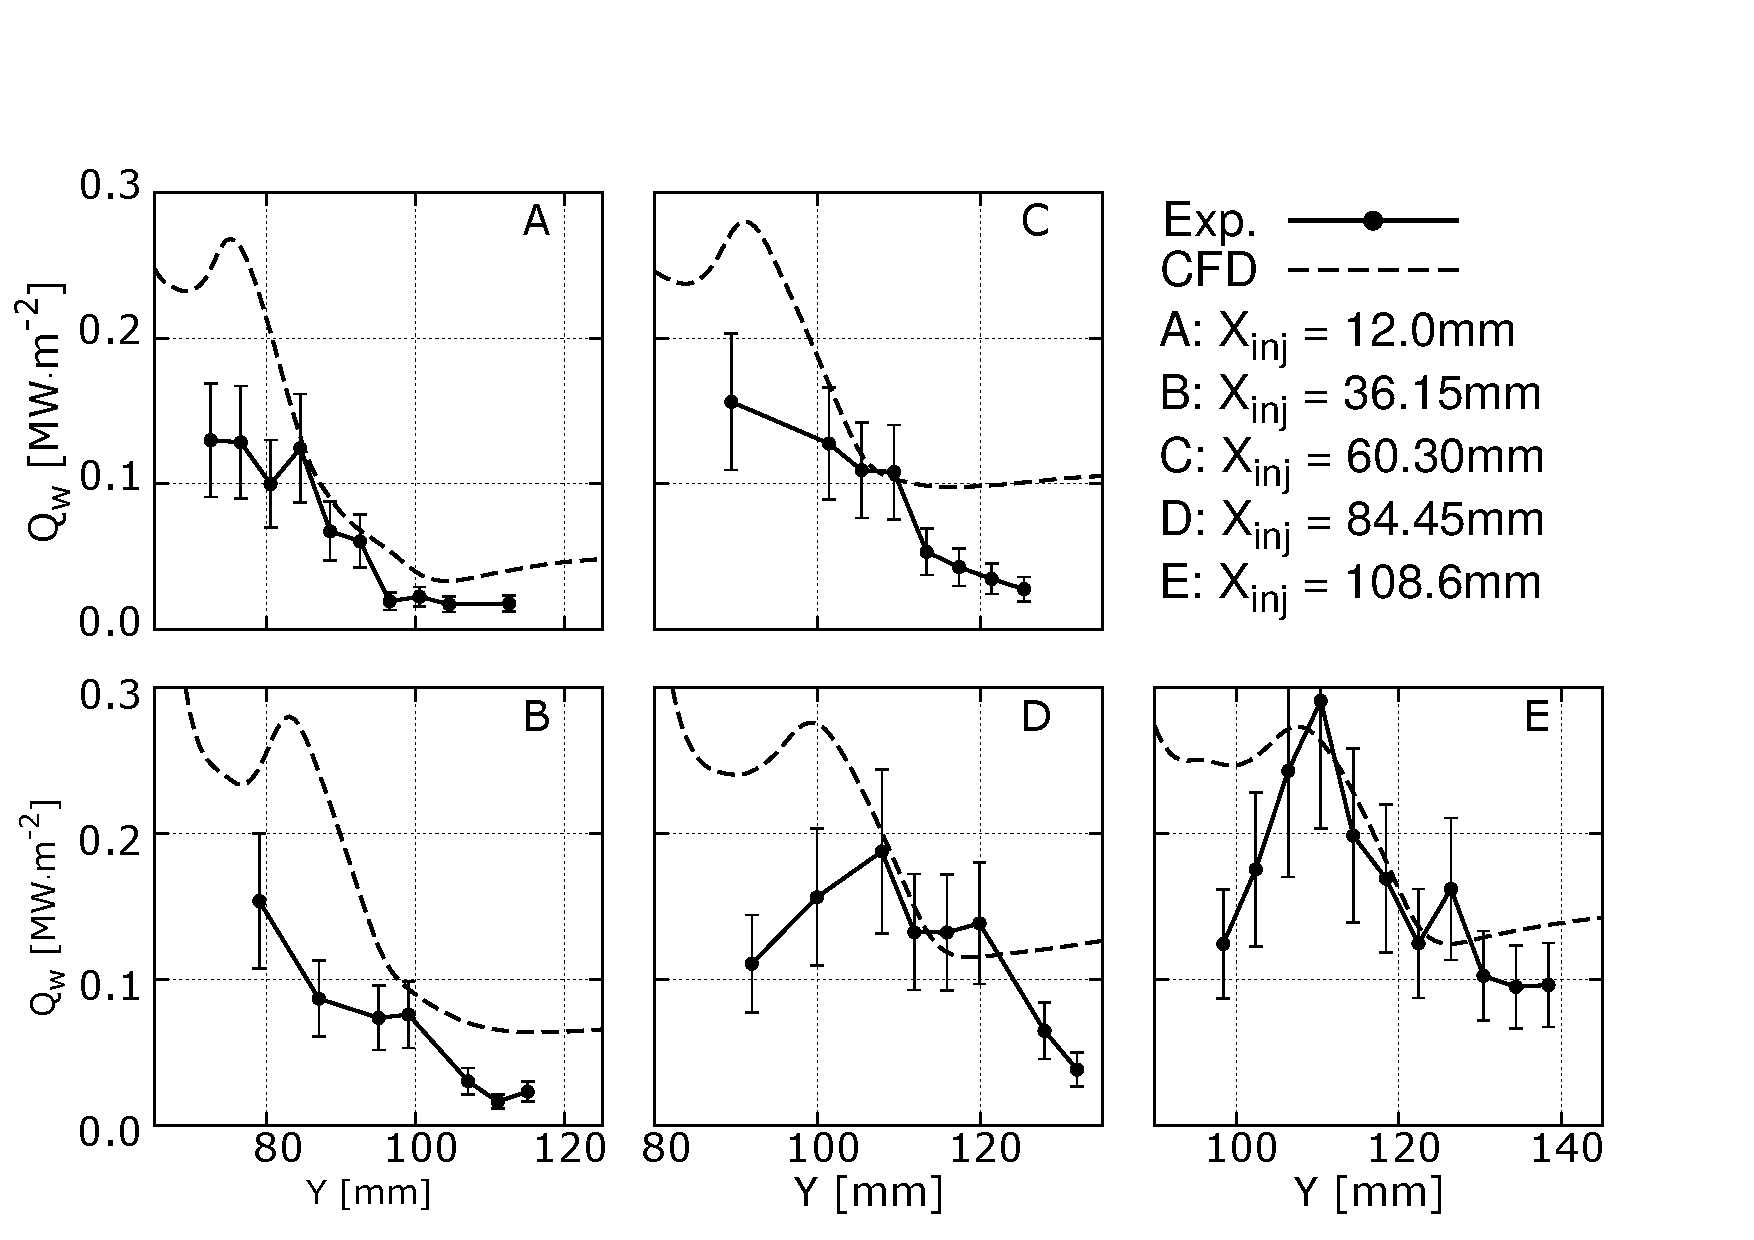
\includegraphics[trim = 0mm 3mm 25mm 25mm, clip, width=0.60\columnwidth,valign=t,fbox]{Figures/Data/LP_NoI_LF/GNUP_CFD_GaugesLines_Multi.pdf}
\label{fig:LP-NI-LF_LinesPlots}
}
%\end{adjustbox}
\caption{Numerical and experimental data on gauges lines A to E, at $X_{inj}$ axial distance from the injector. Unfuelled vortex cases.}
\label{fig:HeatFluxVortex_Lines}
\end{figure} 

The right hand side of the curves in both figures shows a relatively accurate match between the heat flux in the experimental and numerical cases. However, in the region closest to the fin shock (Low Y values), the heat flux is highly overestimated in the numerical results. This overestimation is consistent for all lines. Moreover, the Upper fin case presents a more prominent mismatch in this region. The region of numerically overestimated heat flux lies in the region closer to the fin shock. This can be seen in Fig.~\ref{fig:HeatFluxNILF}, which presents a mapped version of the data in Fig.~\ref{fig:LP-NI-LF_LinesPlots} along with the equivalent numerical data map.

\begin{figure}[!h]
\center
\begin{adjustbox}{max width=1.1\columnwidth,center}
\subfloat[Experimental heat flux map. Solid dots are active gauges. Hollow dots are discarded gauges.]{
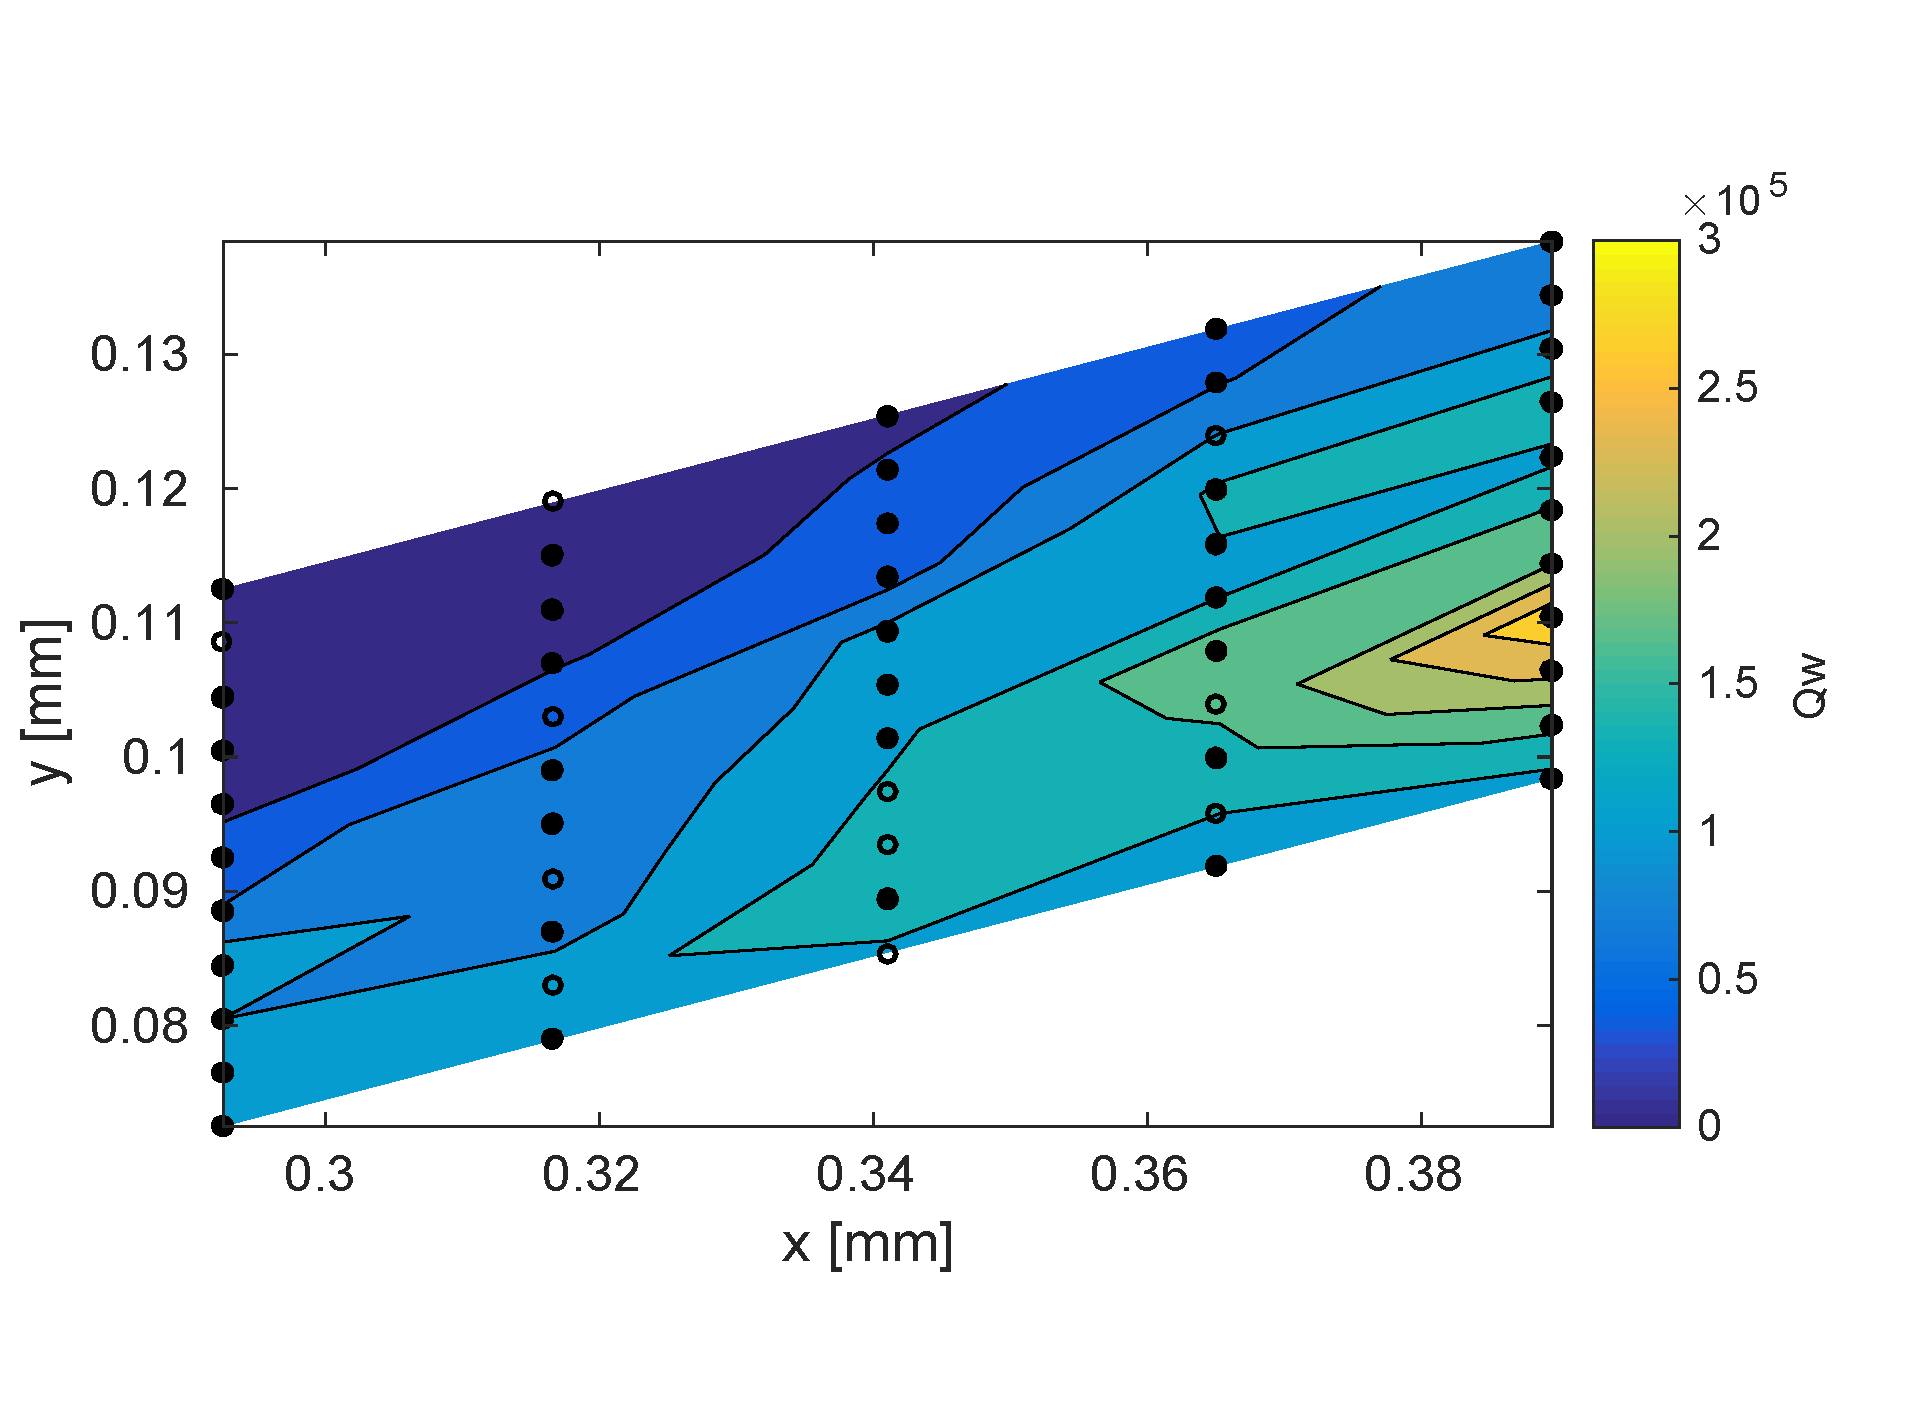
\includegraphics[trim = 0mm 12mm 5mm 12mm, clip, width=0.50\columnwidth,valign=t]{Figures/Data/LP_NoI_LF/Post-processed_GaugesQMap.png}
\label{fig:NI-LF_QwMap}
}
%
\subfloat[Numerical heat flux map. Dotted line indicates experimental acquisition area. Dashed red line indicates separation line. Solid red line indicates location of inviscid fin shock.]{
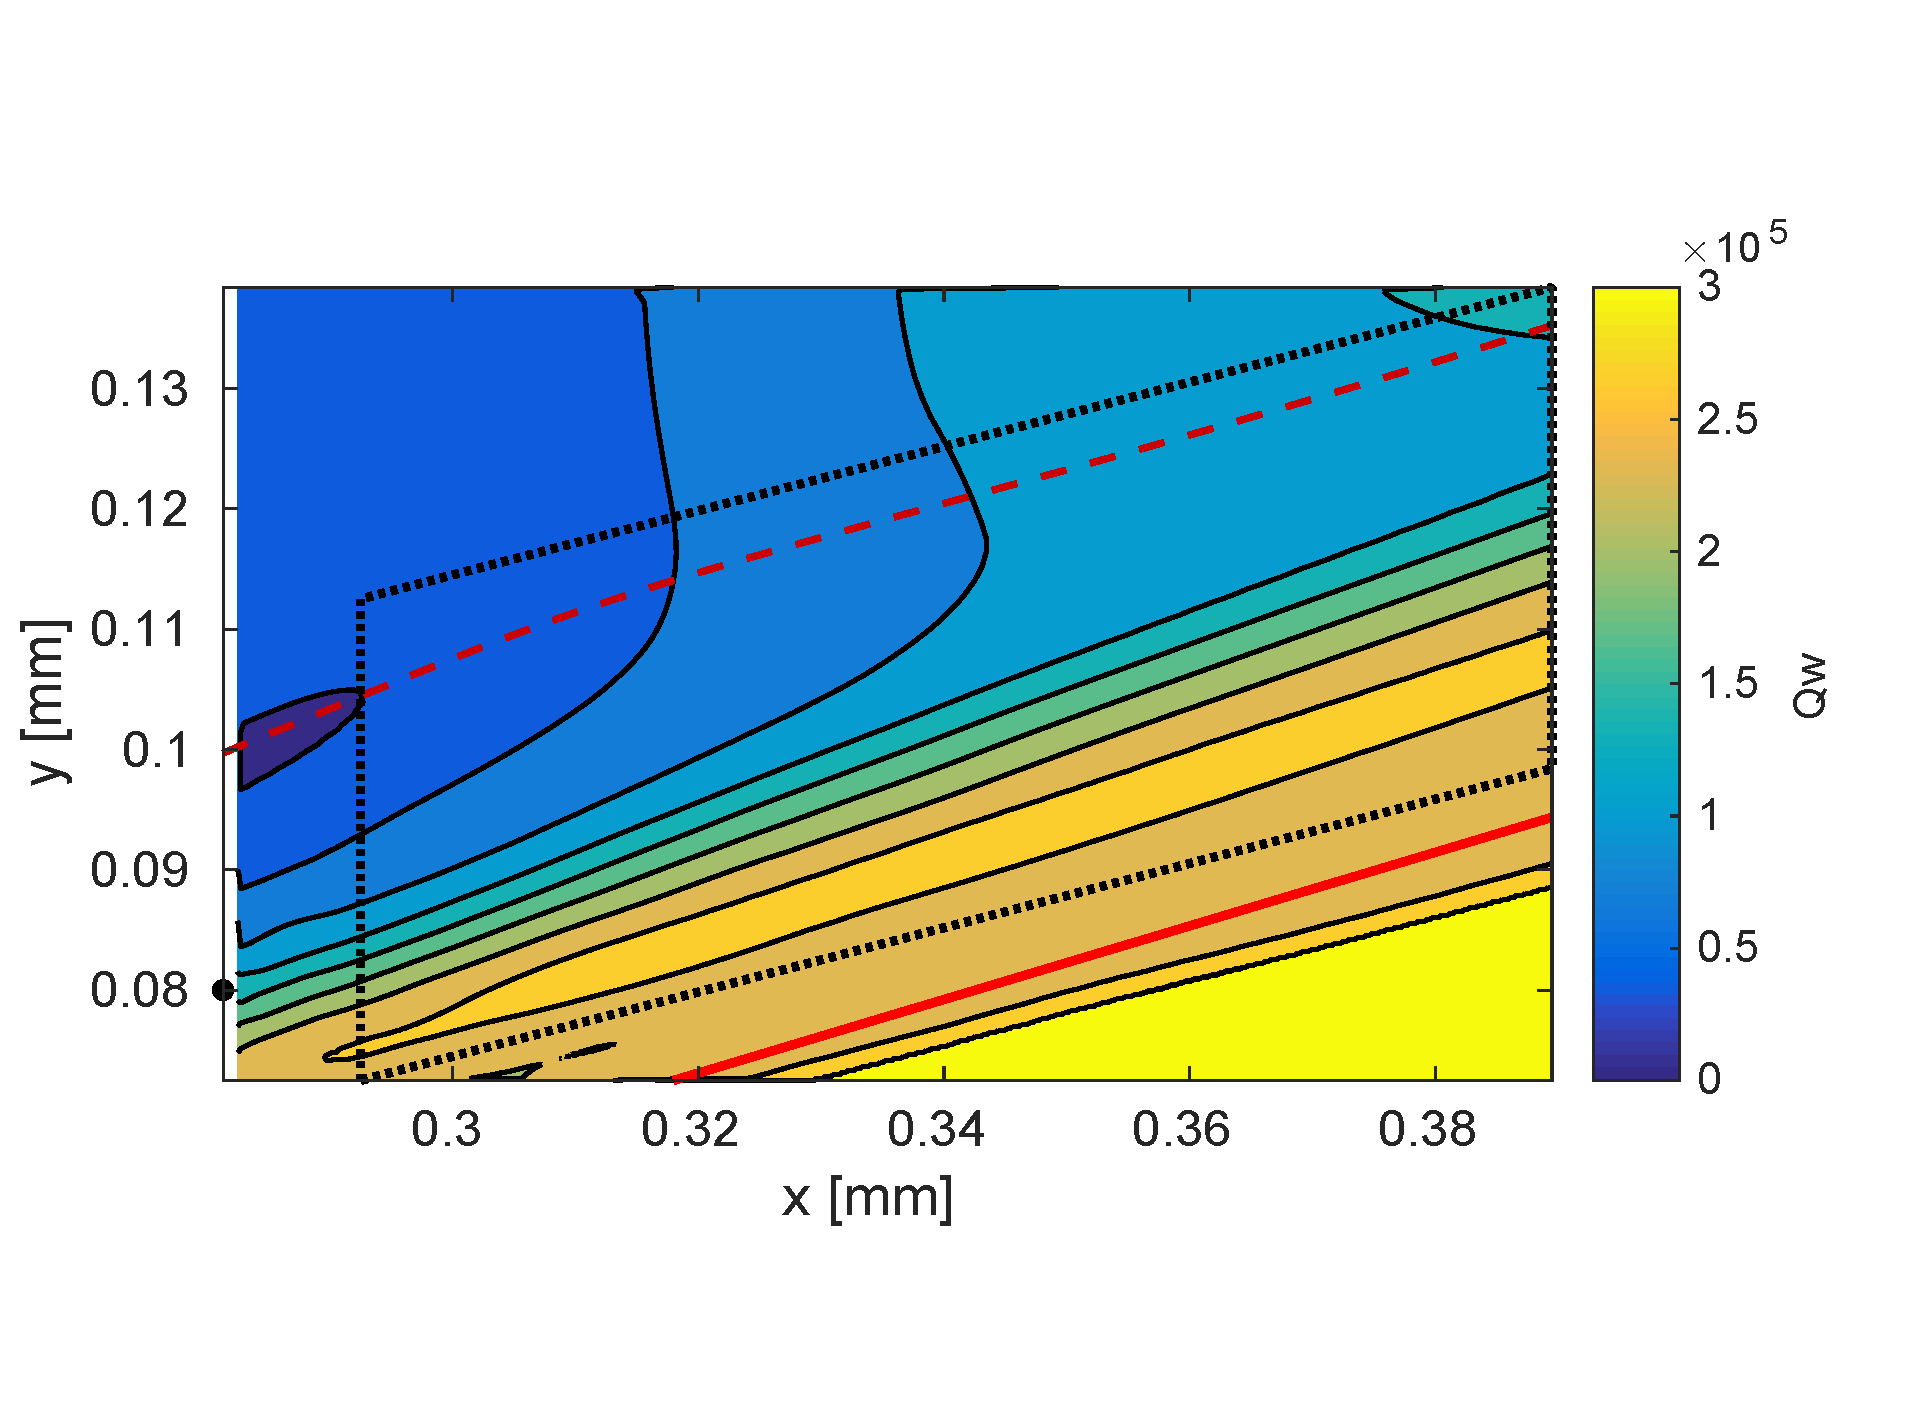
\includegraphics[trim = 0mm 15mm 5mm 17mm, clip, width=0.55\columnwidth,valign=t]{Figures/Data/LP_NoI_LF/Post-processed_CFDB.png}
\label{fig:NI-LF_cfdQwMap}
}
\end{adjustbox}
\caption{Recontructed heat transfer map. Comparison of heat flux from experiments and CFD. NI-LF (Case 2 in Table~\ref{tab:T4_Test_Cases}).}
\label{fig:HeatFluxNILF}
\end{figure} 

In the Lower fin position case, the fin is placed further from the gauge data acquisition region. Therefore, a smaller part of the numerically overpredicted heat flux region is measured experimentally, reducing the discrepancy within the measurement region.

The vortex flowfield contains a separation and a reattachment line. The reattachment takes place behind the fin shock, driving hot and dense shock processed gas towards the flat plate, as observed in Fig~\ref{fig:Alvi_Sketch} marked as 'jet'. This reattachment takes place in the region of numerically overestimated heat flux. Assuming the temperature of the gas and its composition after being processed by the fin shock are accurately predicted numerically, the overestimation of heat flux seems to be caused by an overestimation of the turbulence intensity in the reattachment region. This can be observed in Fig.~\ref{fig:SSTk_Q_Combi}. This figure shows line A from the Upper fin case (Fig.~\ref{fig:LP-NI-UF_LinesPlots}) combined with the turbulent kinetic energy at the same axial location extracted from the numerical data. The location where the numerical overestimation becomes severe is coincident with the start of a region of high turbulent kinetic energy adjacent to the flat plate surface. The detail image in Fig.~\ref{fig:SSTk_Q_Combi} clearly shows this region. The coincidence between the overestimation area with the high turbulent kinetic energy adjacent to the flat plate suggests the turbulence model is overpredicting turbulence and thus heat flux in this region.
%
\begin{figure}[!h]
\center
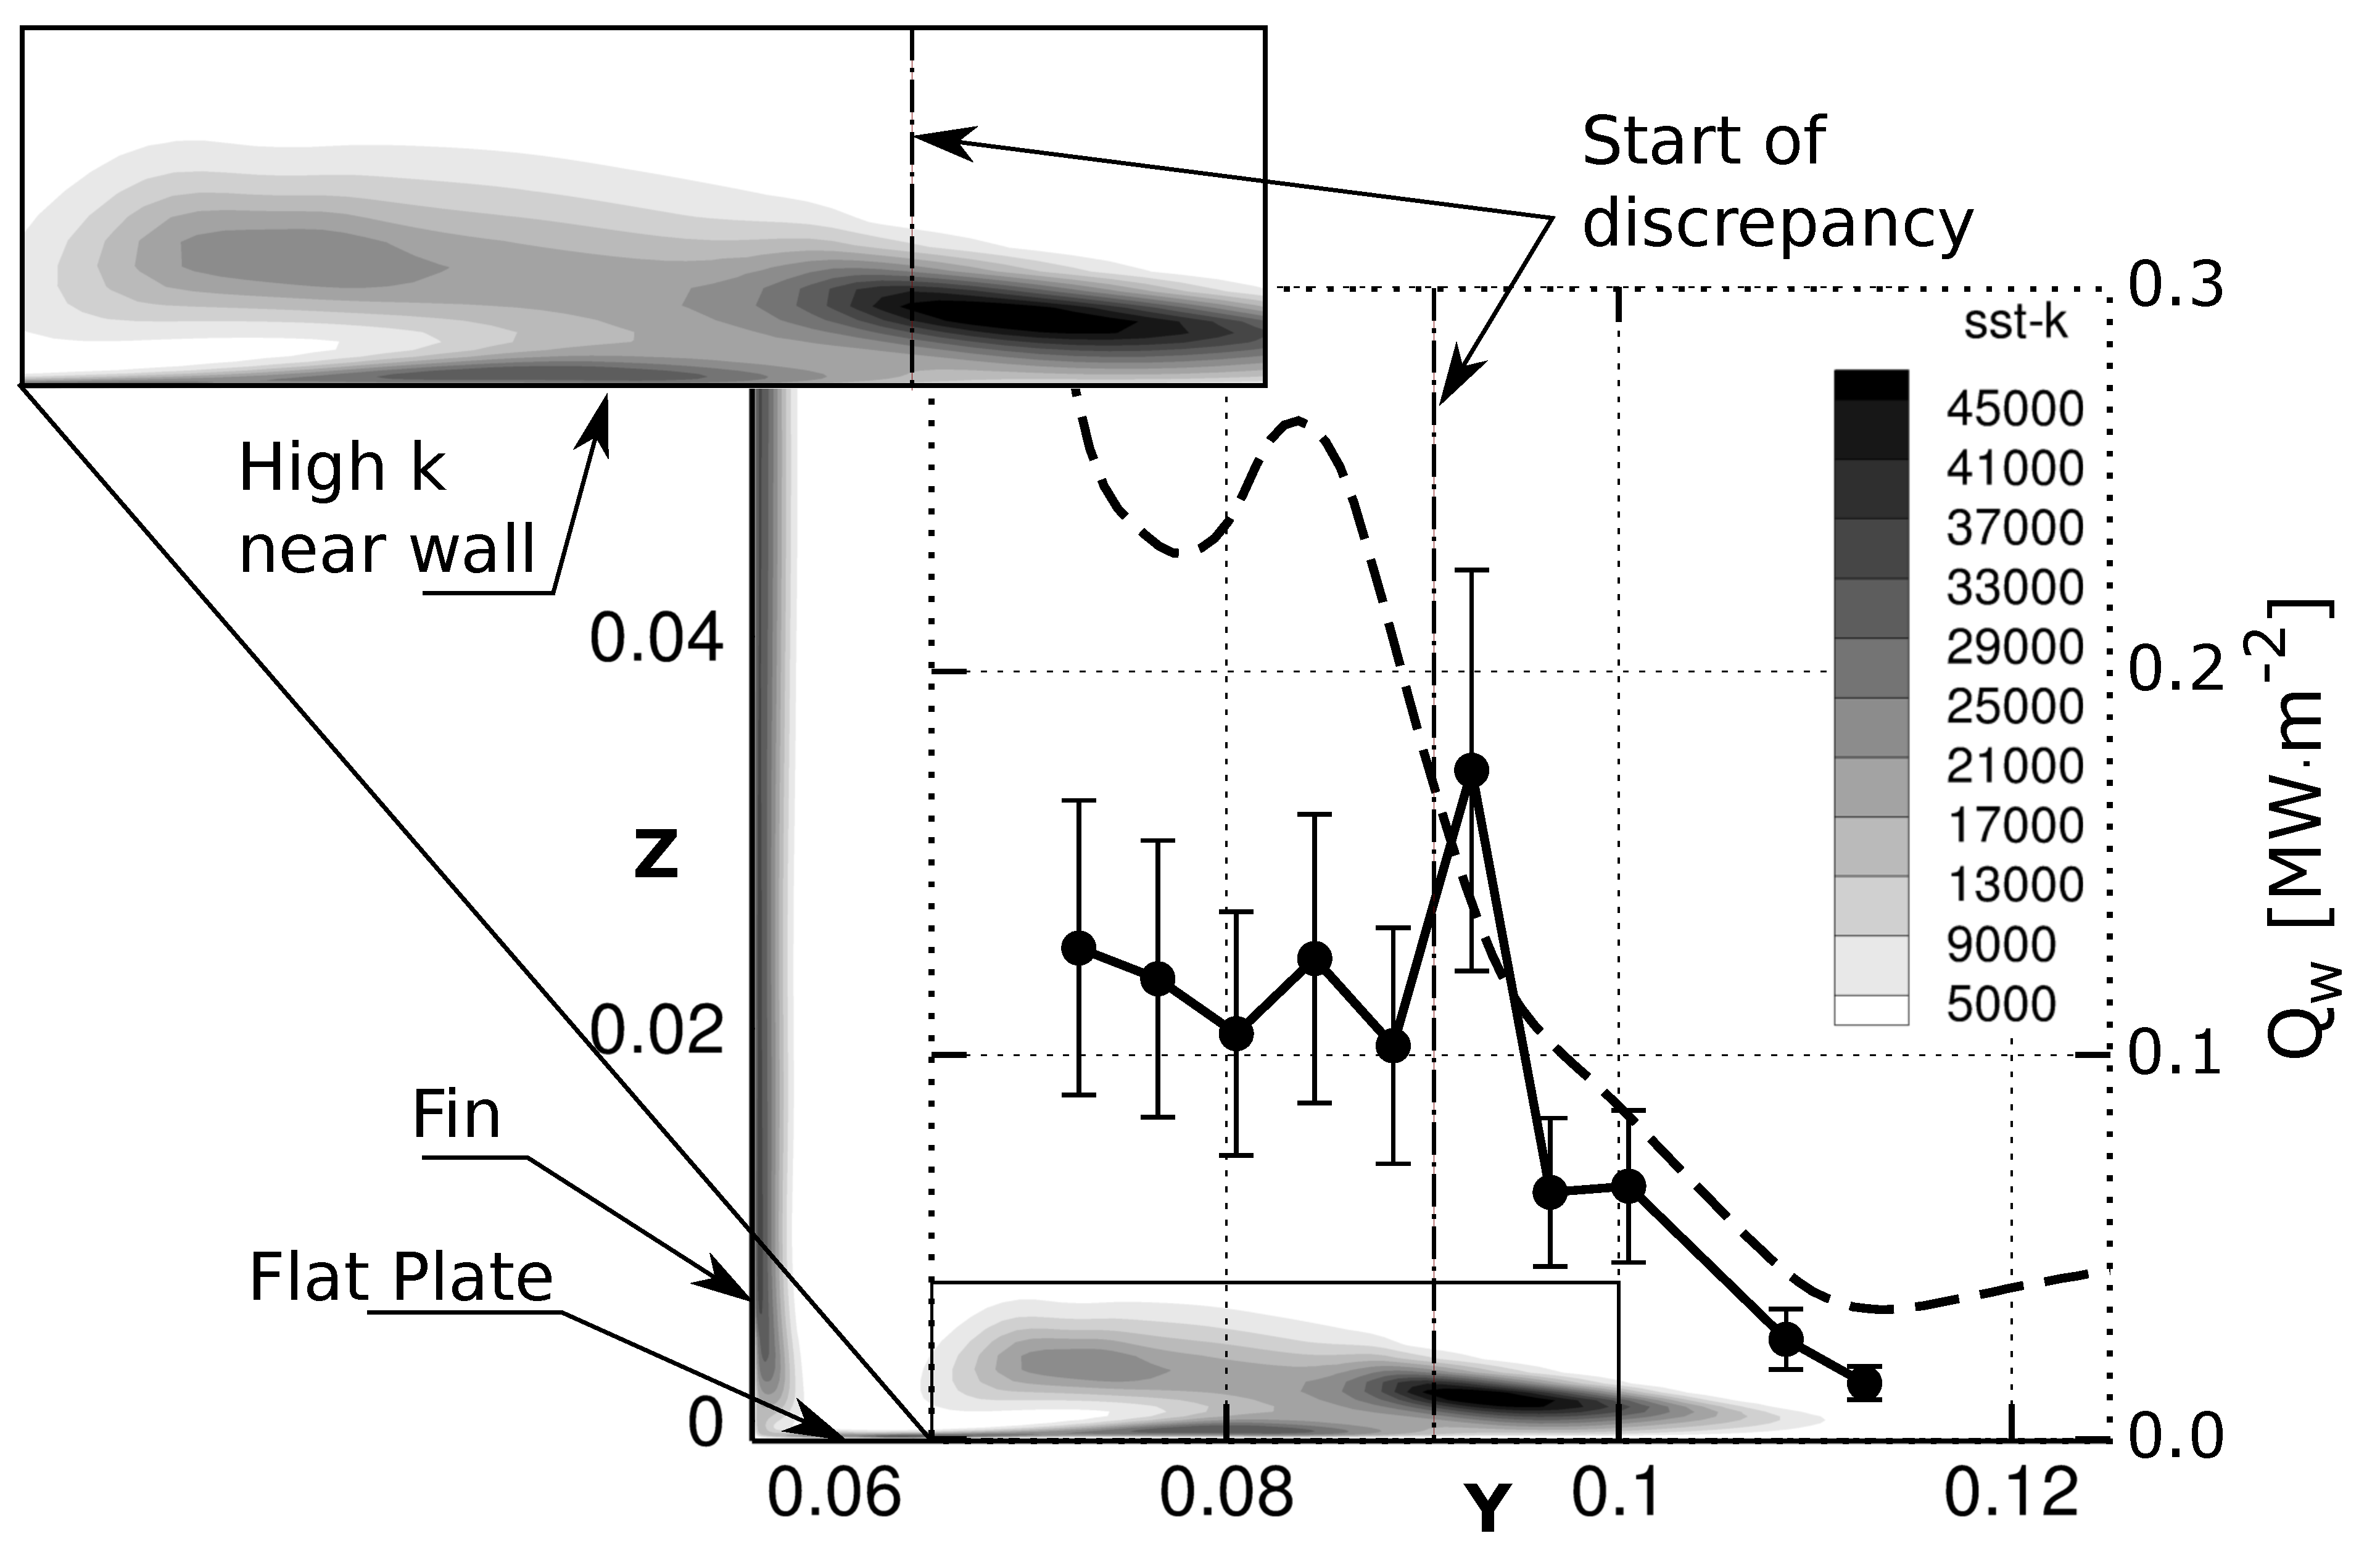
\includegraphics[width=0.70\columnwidth,valign=t]{Figures/SST-K_X137_LP_NI_UF_Q_and_SSTk_Combined.pdf}
\caption{Contours of turbulent kinetic energy combined with experimental and numerical heat flux at $X_{inj} = \SI{12}{\milli\meter}$.}
\label{fig:SSTk_Q_Combi}
\end{figure} 

The limitation of the numerical model to accurately simulate heat flux near the fin shock is a key aspect to take into account when comparing the numerical and experimental results for the fueled cases. 
This region of severe heat flux overprediction in the numerical data will be referred as `numerical overestimation zone'.


%%%%%%%%%%%%%%%%%%%%
\subsection{Fuel vortex interaction}

The results obtained for the tests using the Upper and Lower fin positions in combination with the high and low injection pressures (cases 1-4 in Table~\ref{tab:T4_Test_Cases}) provide data on the complex vortex-injection interaction flow field.


\subsubsection{Upper fin position, High injection pressure}

Both the experimental and numerical results for the high injection pressure and upper fin are presented in Fig.~\ref{fig:HeatFluxLPHIUF}. Qualitatively, very good agreement between the numerical and experimental results is achieved. The general shape of the curves is well matched. The location of the heat flux peaks induced by the injection bow shock is very accurately retrieved numerically. Moreover, the similarity between numerical and experimental heat flux values is very satisfactory except in the region closest to the fin shock (low Y values). Near the fin shock, the numerical heat flux shows an important overestimation. This is caused by the presence of the `numerical overestimation zone' previously described. As seen in Fig.~\ref{fig:SSTk_Q_Combi}, the turbulent kinetic energy adjacent to the flat plate wall, near the fin shock, tends to be overestimated. This not only affects the regions unaffected by the injection bow shock, but also contributes to increase the value of the peaks within this region, as can be seen in Line A. 

%
%LP_HI_UF
\begin{figure}[!h]
\center
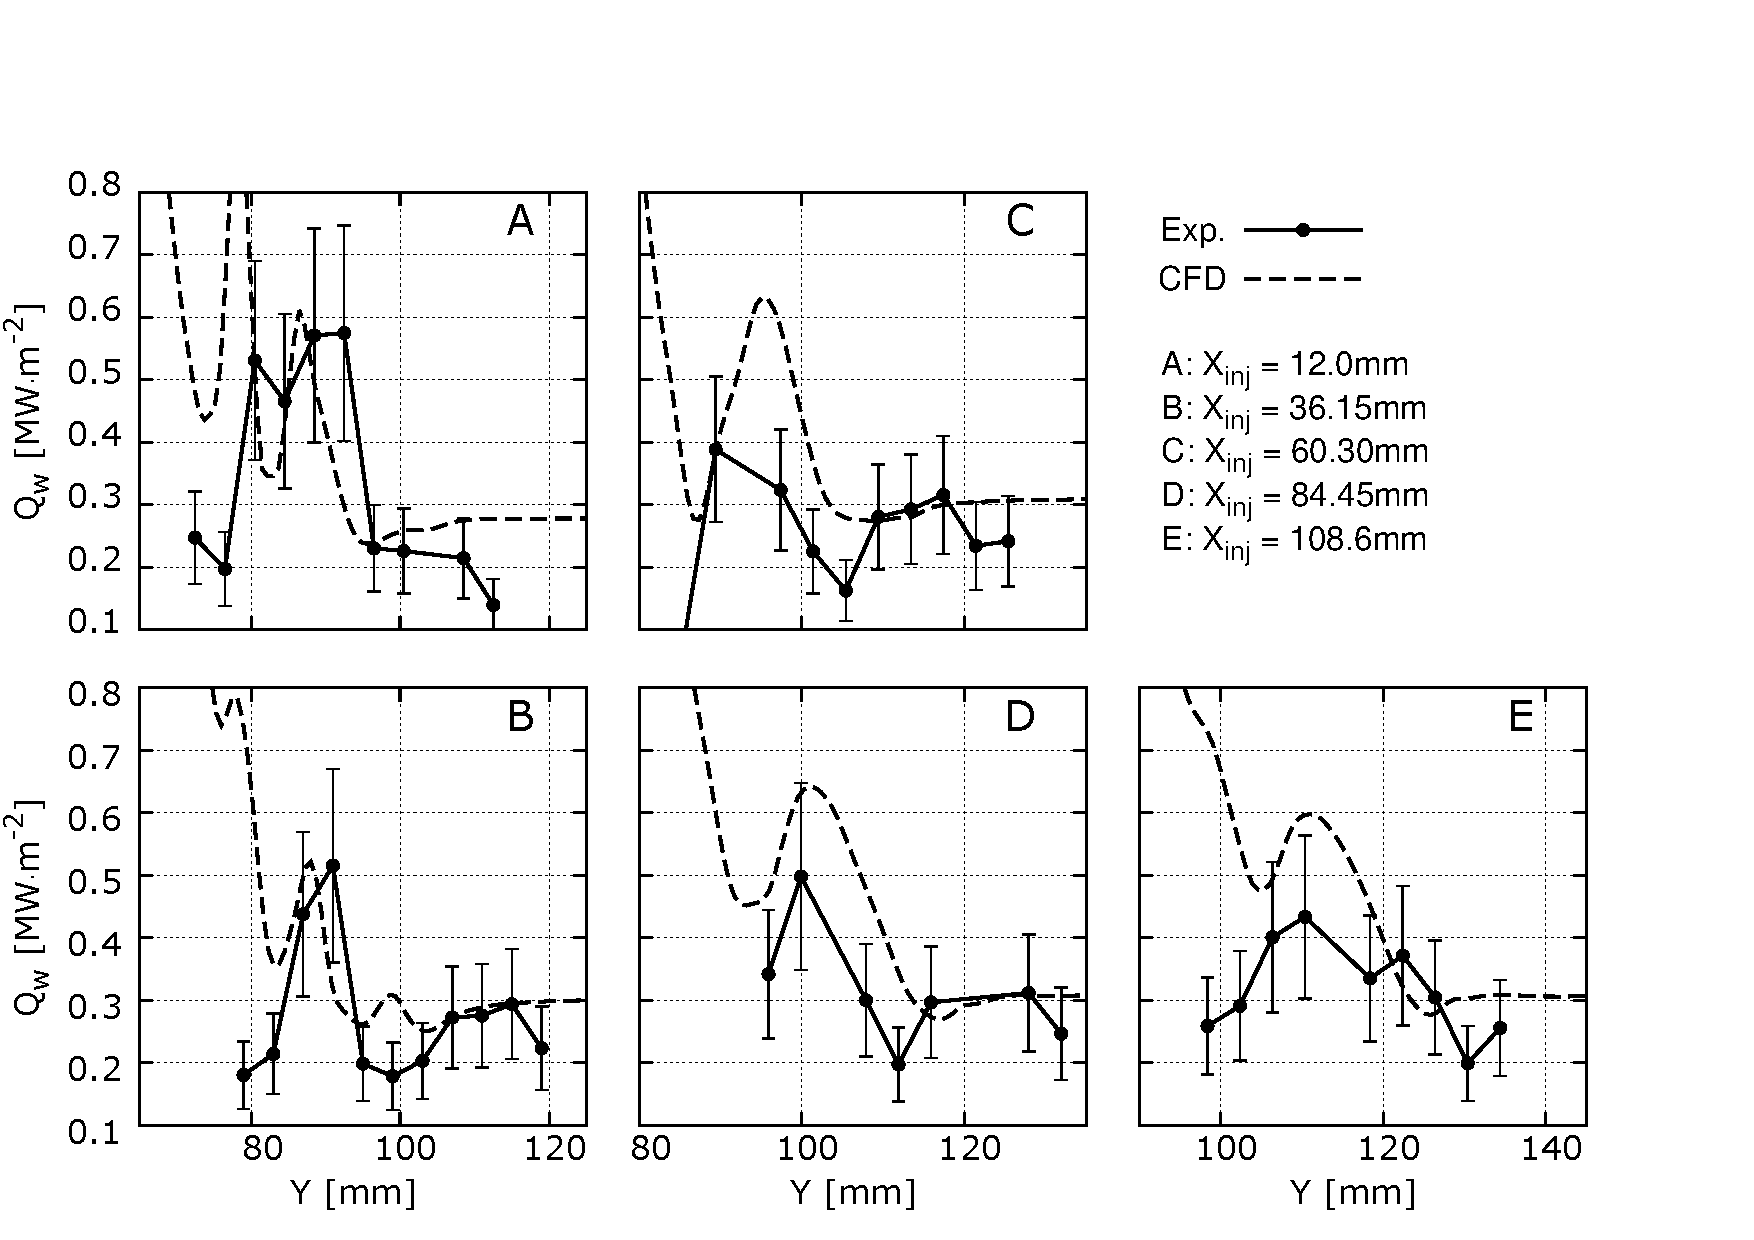
\includegraphics[trim = 0mm 3mm 25mm 25mm, clip, width=0.60\columnwidth,valign=t,fbox]{Figures/Data/LP_HI_UF/GNUP_CFD_GaugesLines_Multi.pdf}
\caption{Numerical and experimental heat transfer data. HI-UF (Case 1 in Table~\ref{tab:T4_Test_Cases})}
\label{fig:HeatFluxLPHIUF}
\end{figure} 


\begin{figure}[!h]
\center
\begin{adjustbox}{max width=1.1\columnwidth,center}
\subfloat[Experimental heat flux map. Solid dots are active gauges. Hollow dots are discarded gauges.]{
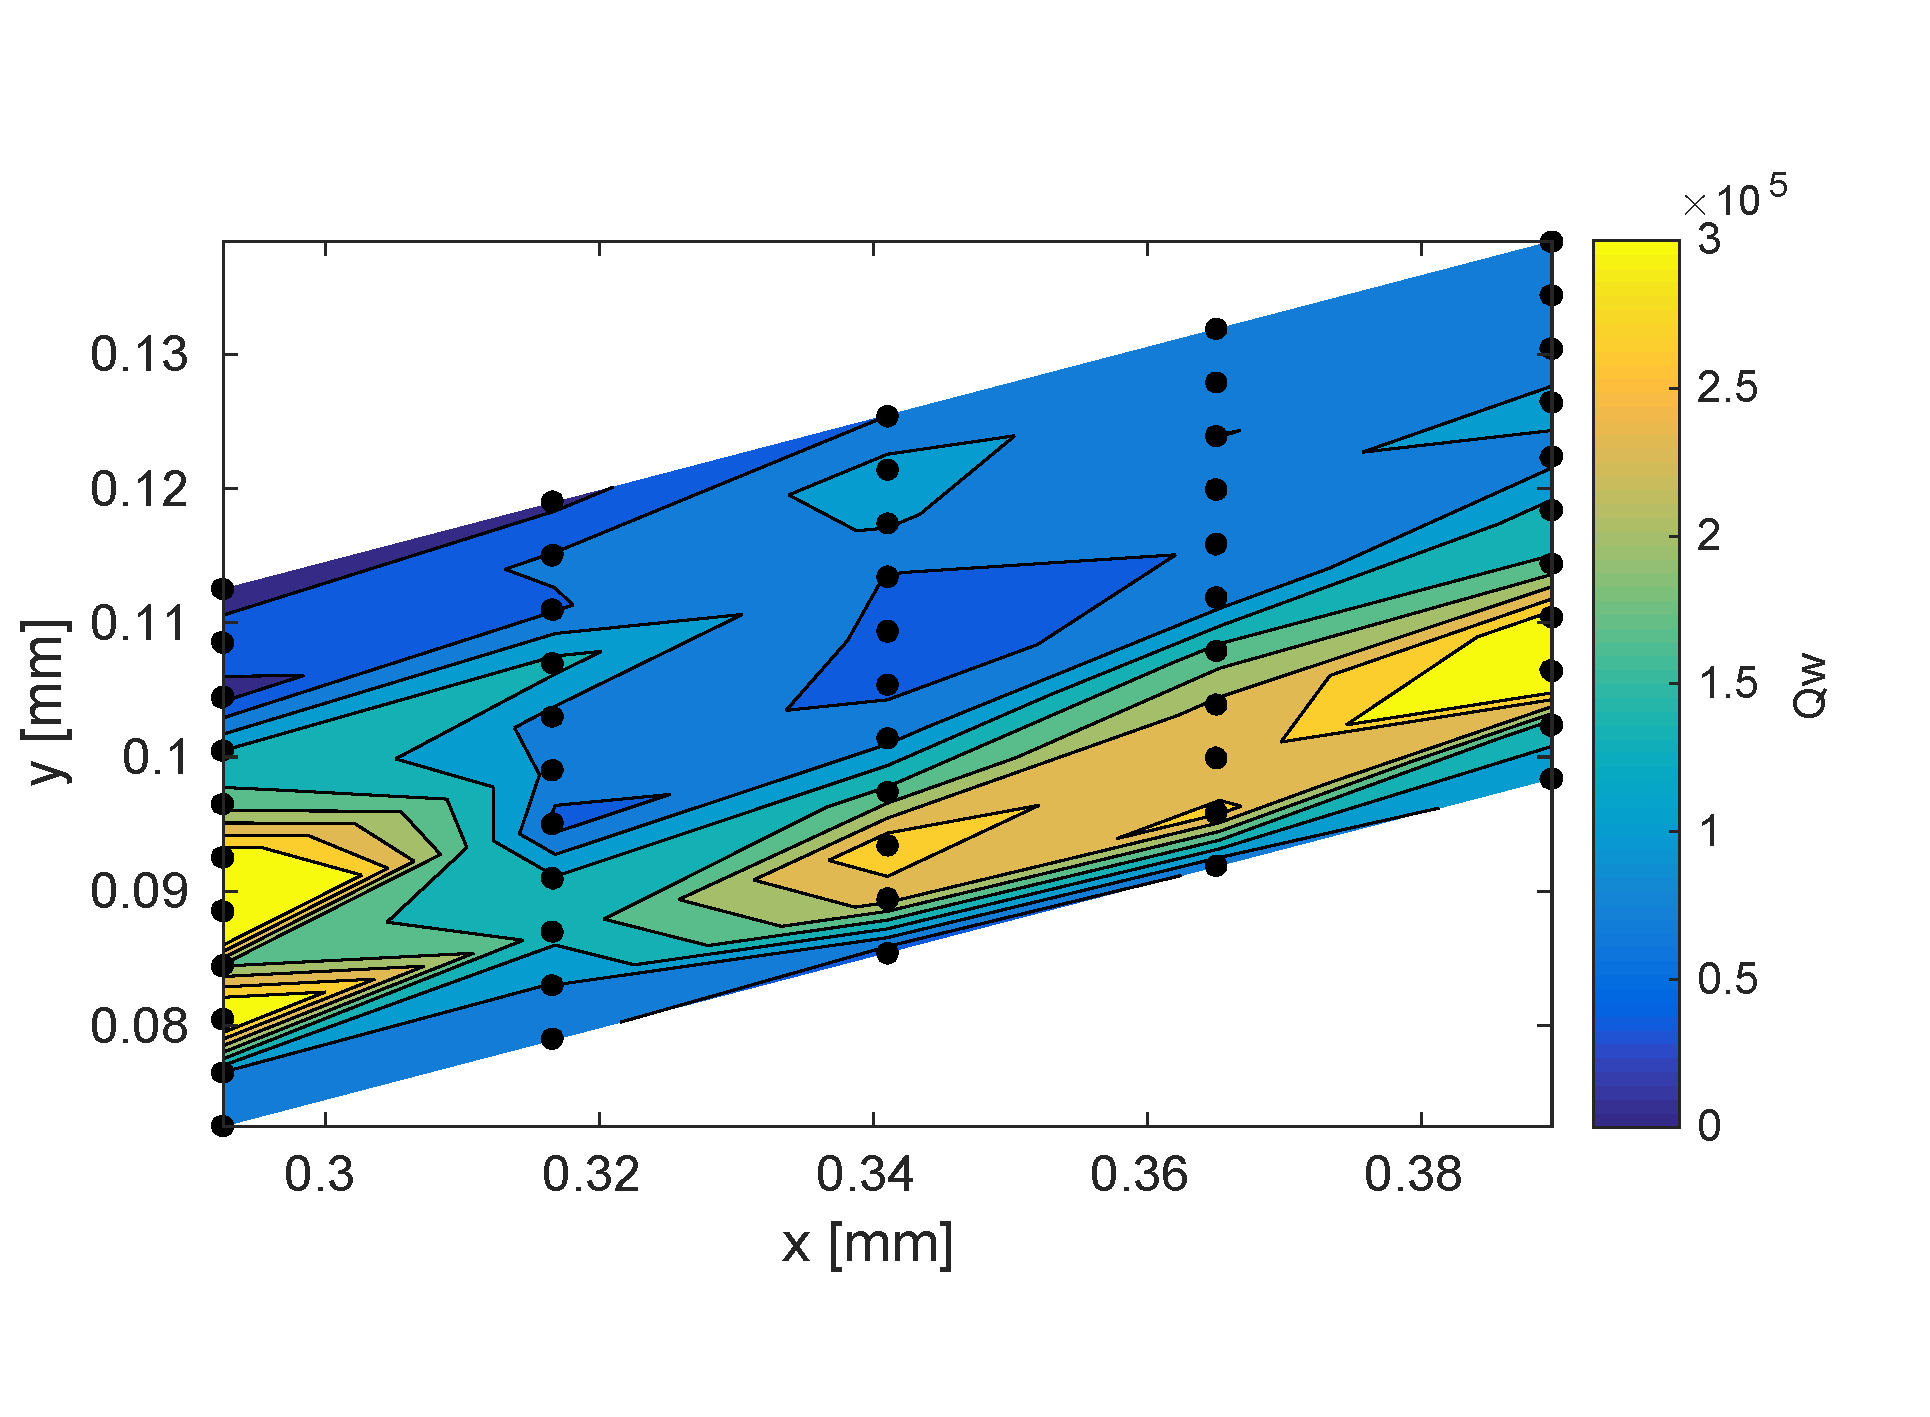
\includegraphics[trim = 0mm 12mm 5mm 12mm, clip, width=0.50\columnwidth,valign=t]{Figures/Data/LP_HI_UF/Post-processed_GaugesQMap.png}
\label{fig:LP-HI-UF_QwMap}
}
%
\subfloat[Numerical heat flux map. Dotted line indicates experimental acquisition area. Dashed red line indicates separation line. Solid red line indicates location of inviscid fin shock.]{
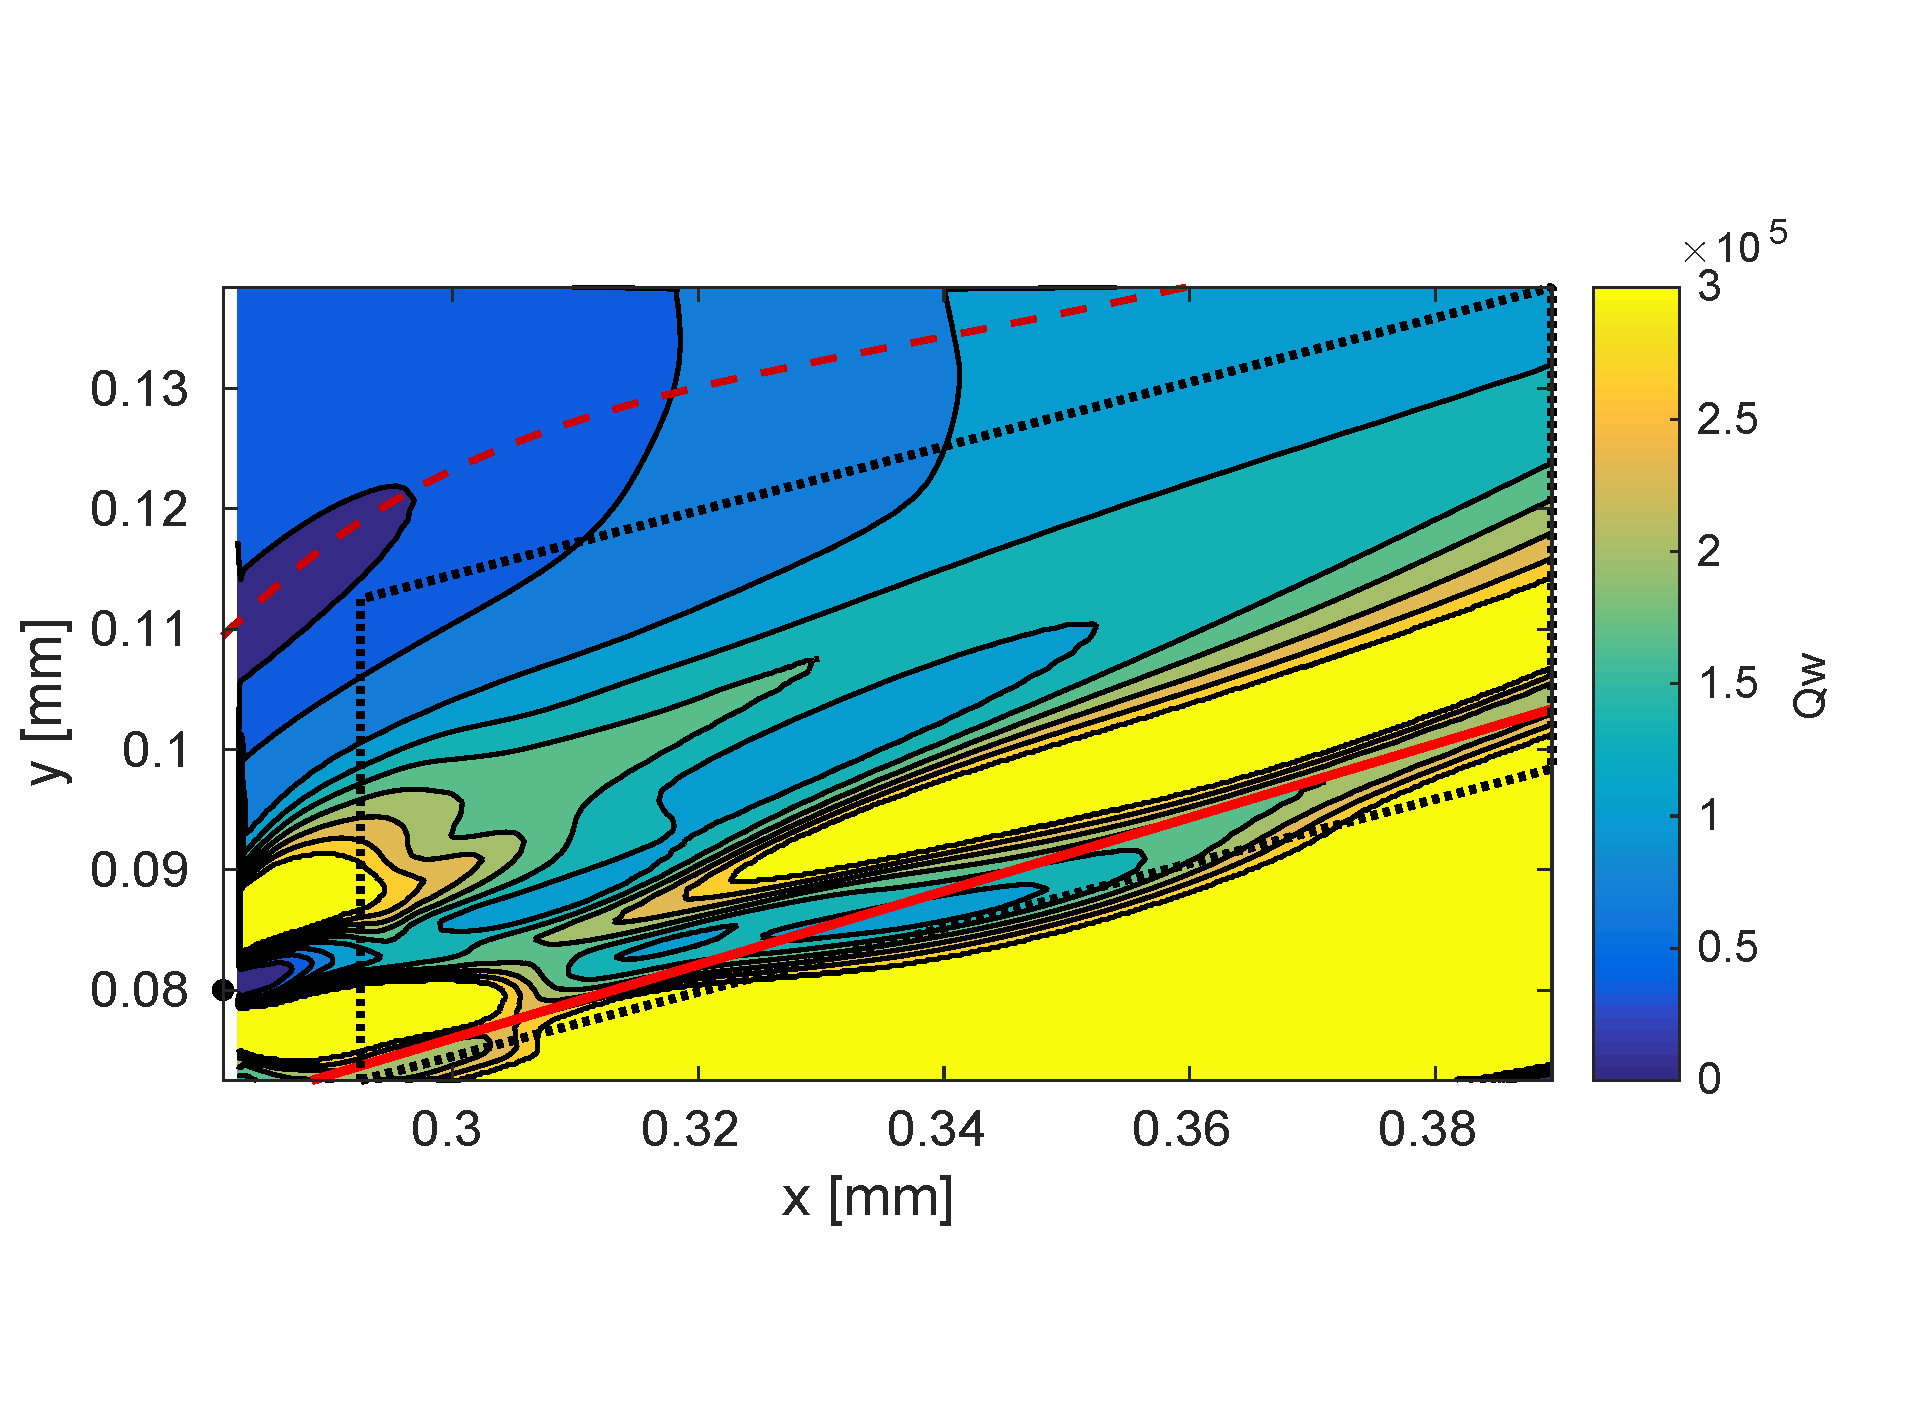
\includegraphics[trim = 0mm 15mm 5mm 17mm, clip, width=0.55\columnwidth,valign=t]{Figures/Data/LP_HI_UF/Post-processed_CFDB.png}
\label{fig:LP-HI-UF_cfdQwMap}
}
\end{adjustbox}
\caption{Recontructed heat transfer map. Comparison of heat flux from experiments and CFD. HI-UF (Case 3 in Table~\ref{tab:T4_Test_Cases})}
\label{fig:HeatFluxMap}
\end{figure} 


\subsubsection{Flowfield description from numerical data}

The heat flux distribution on the flat plate present an interesting feature consisting of a stripe of high heat flux approximately in the center of the vortex. This regions extends from shortly downstream of the injection bow shock up to the end of the measurement region. This feature is difficult to visualize in the curves in Fig.~\ref{fig:HeatFluxLPHIUF}, but it is apparent in the heat flux maps in Fig.~\ref{fig:HeatFluxMap}. This high heat flux stripe is coupled with a neighboring low heat flux stripe, both highlighted in Fig.~\ref{fig:Exper_Flowf}. Fig.~\ref{fig:Exper_Flowf} presents the numerical data showing the vortex-injection interaction flowfield. 

Fig.~\ref{fig:Exper_Flowf}a shows the evolution of the flow from upstream of the injector, to far downstream. The fuel plume evolves from a nearly hemispheric, to a highly elongated profile. Far downstream, the fuel plume splits in two regions, one located within the vortex recirculation region, and the other adjacent to the flat plate. The region of interest is presented in more detail in Fig.~\ref{fig:Exper_Flowf}b. In this figure, the streak lines on the flat plate surface show the high and low heat flux stripes are coincident with a separation and a reattachment of the flow. The separation and reattachment lines are linked to the existence of a counter rotating vortex in this region. This vortex is shown in Fig.~\ref{fig:Exper_Flowf}c, marked as `C.R. vortex'.

\begin{figure}[!h]
\center
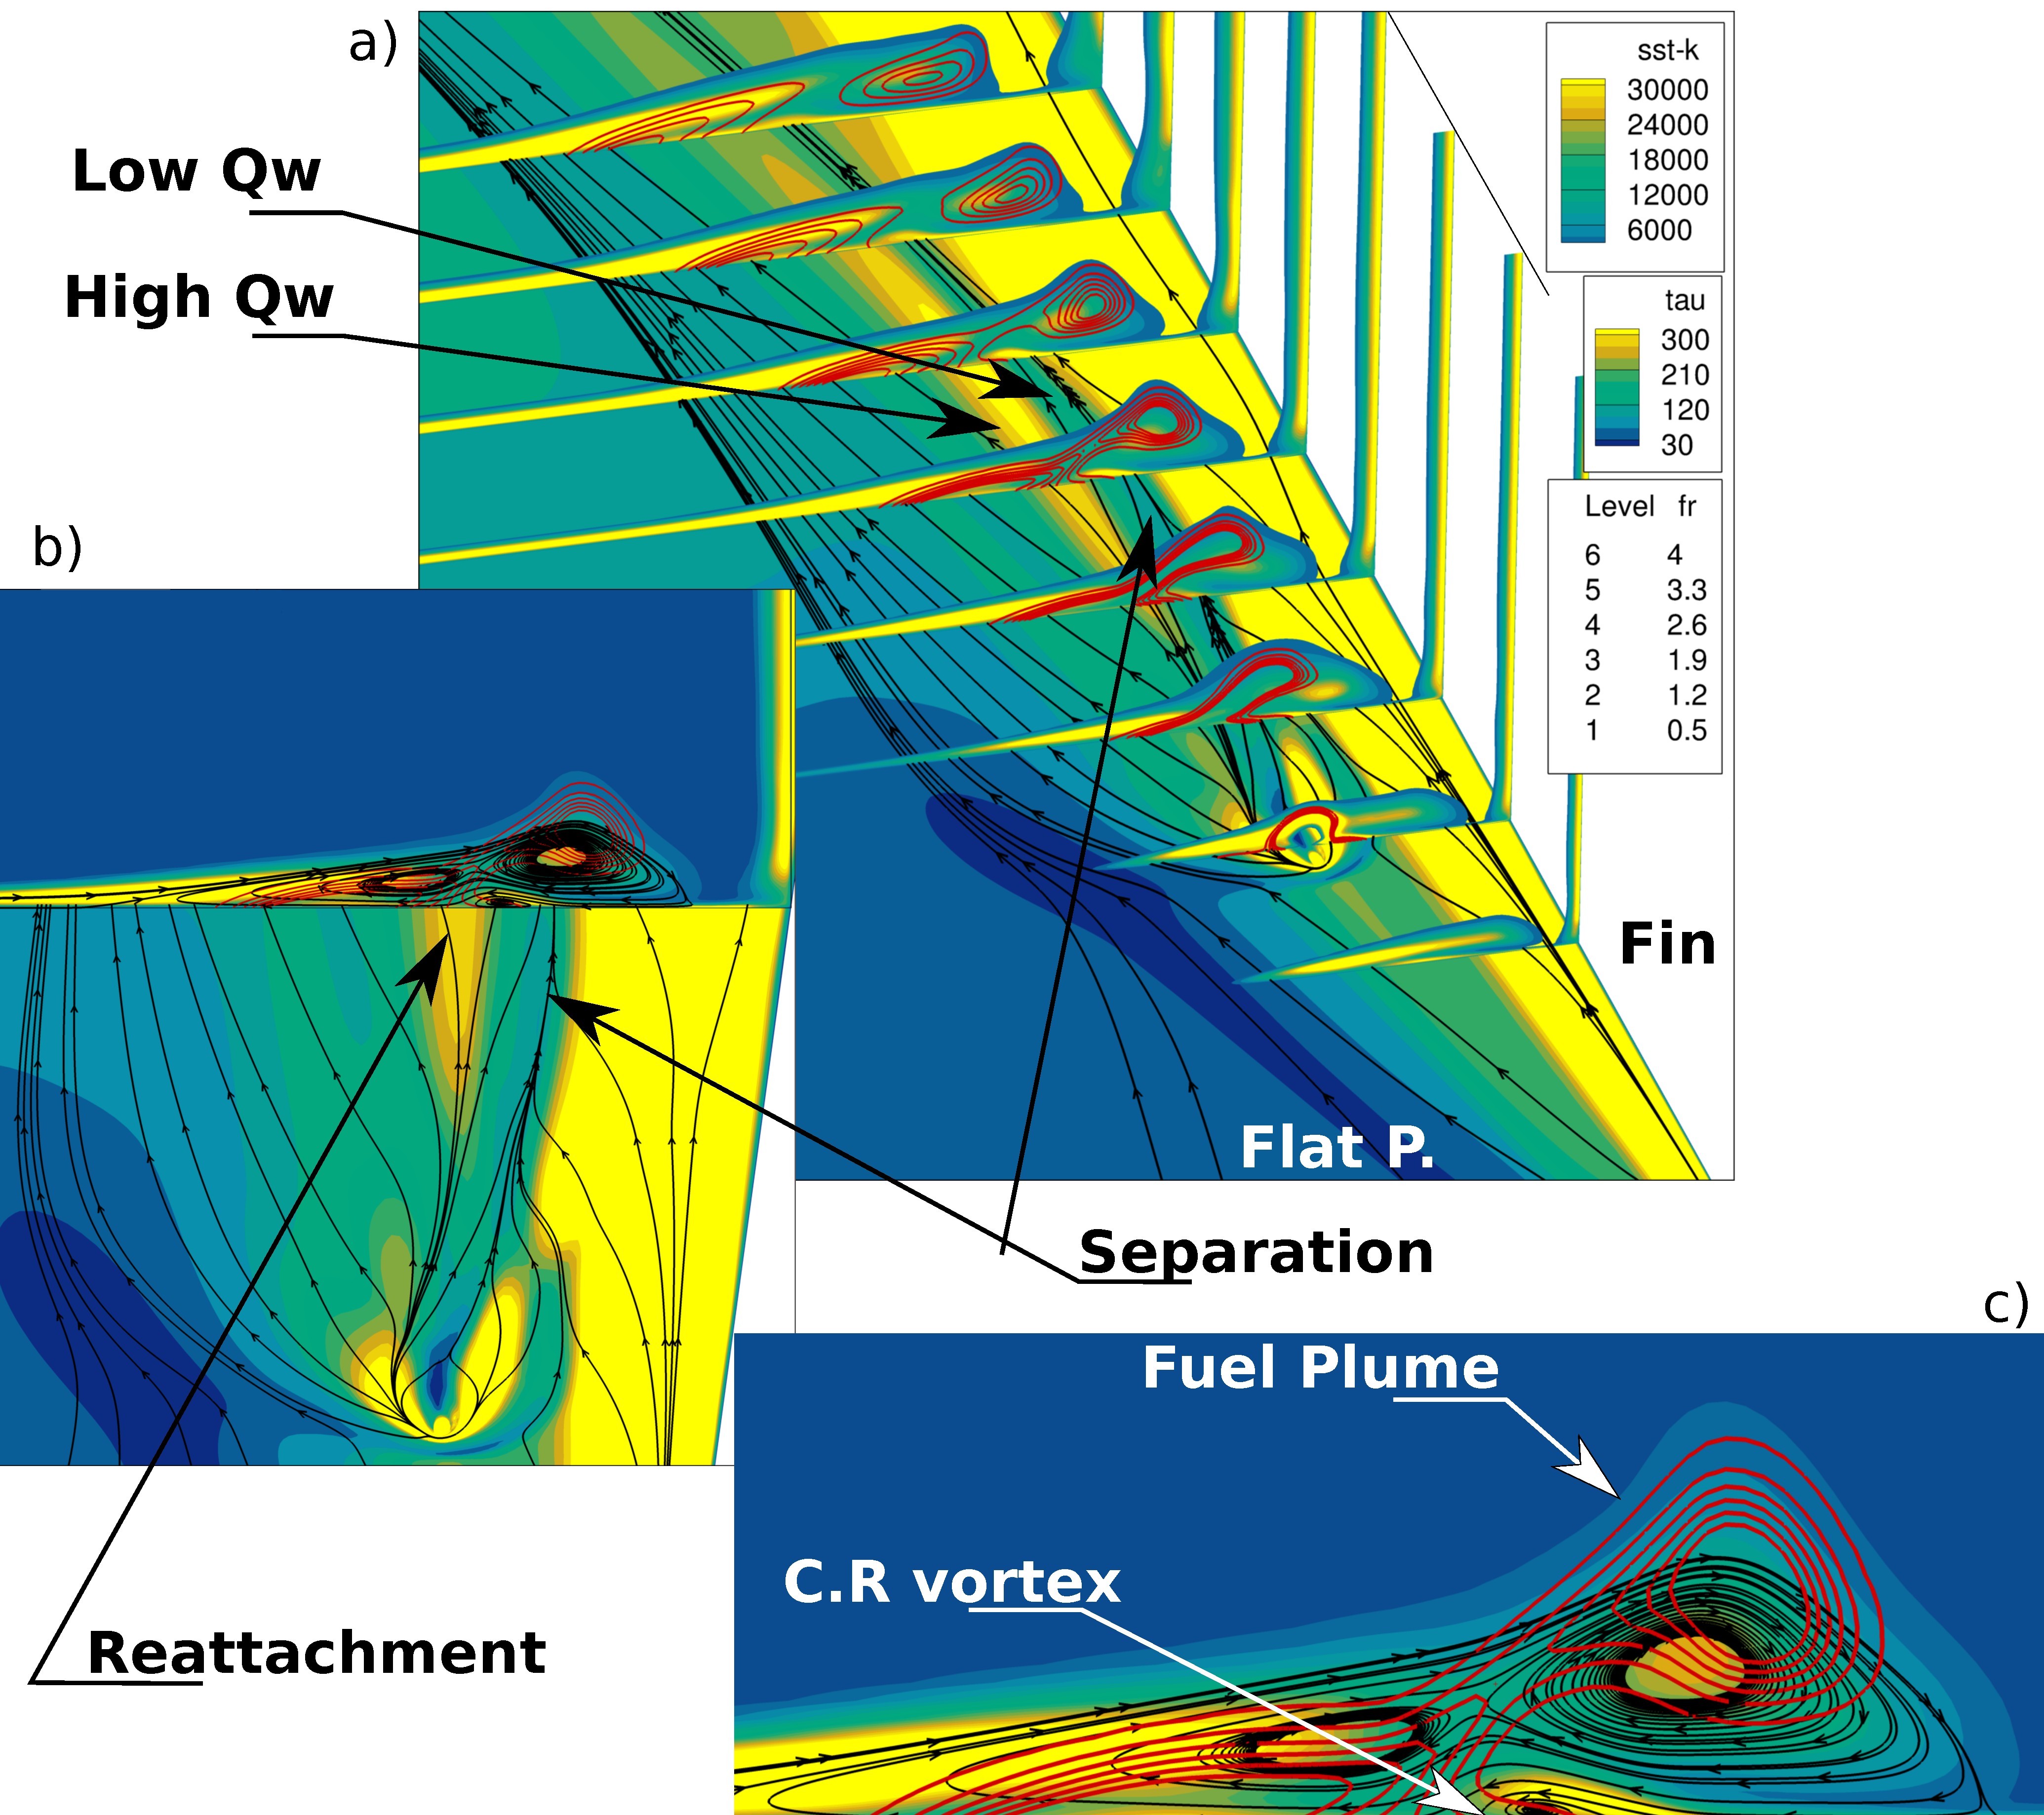
\includegraphics[trim = 0mm 0mm 0mm 0mm, clip, width=0.95\columnwidth,valign=t]{Figures/Flowfield_Experimental_Vred.pdf}
\caption{Flat plate surface: numerical heat flux map with streak-lines. Slices: contours of turbulent kinetic energy, lines of equivalence ratio (red), and surface streamtraces. LP-HI-UF case.}
\label{fig:Exper_Flowf}
\end{figure} 

Despite the localized region of heat flux overprediction previously observed, the ability of the numerical methodology to accurately predict the location and extent of the counter-rotating vortex within the main separation vortex indicates the 3-D flowfield is very accurately predicted.

\subsubsection{Upper fin position, Low injection pressure}

The case with low injection pressure shows very similar results to the high injection case. The location of the heat flux peaks is again very well predicted numerically. Moreover, the region far from the fin shock shows fairly good agreement in heat flux level.
This can be observed in Fig.~\ref{fig:HeatFluxLPLIUF}

%LP_LI_UF
\begin{figure}[!h]
\center
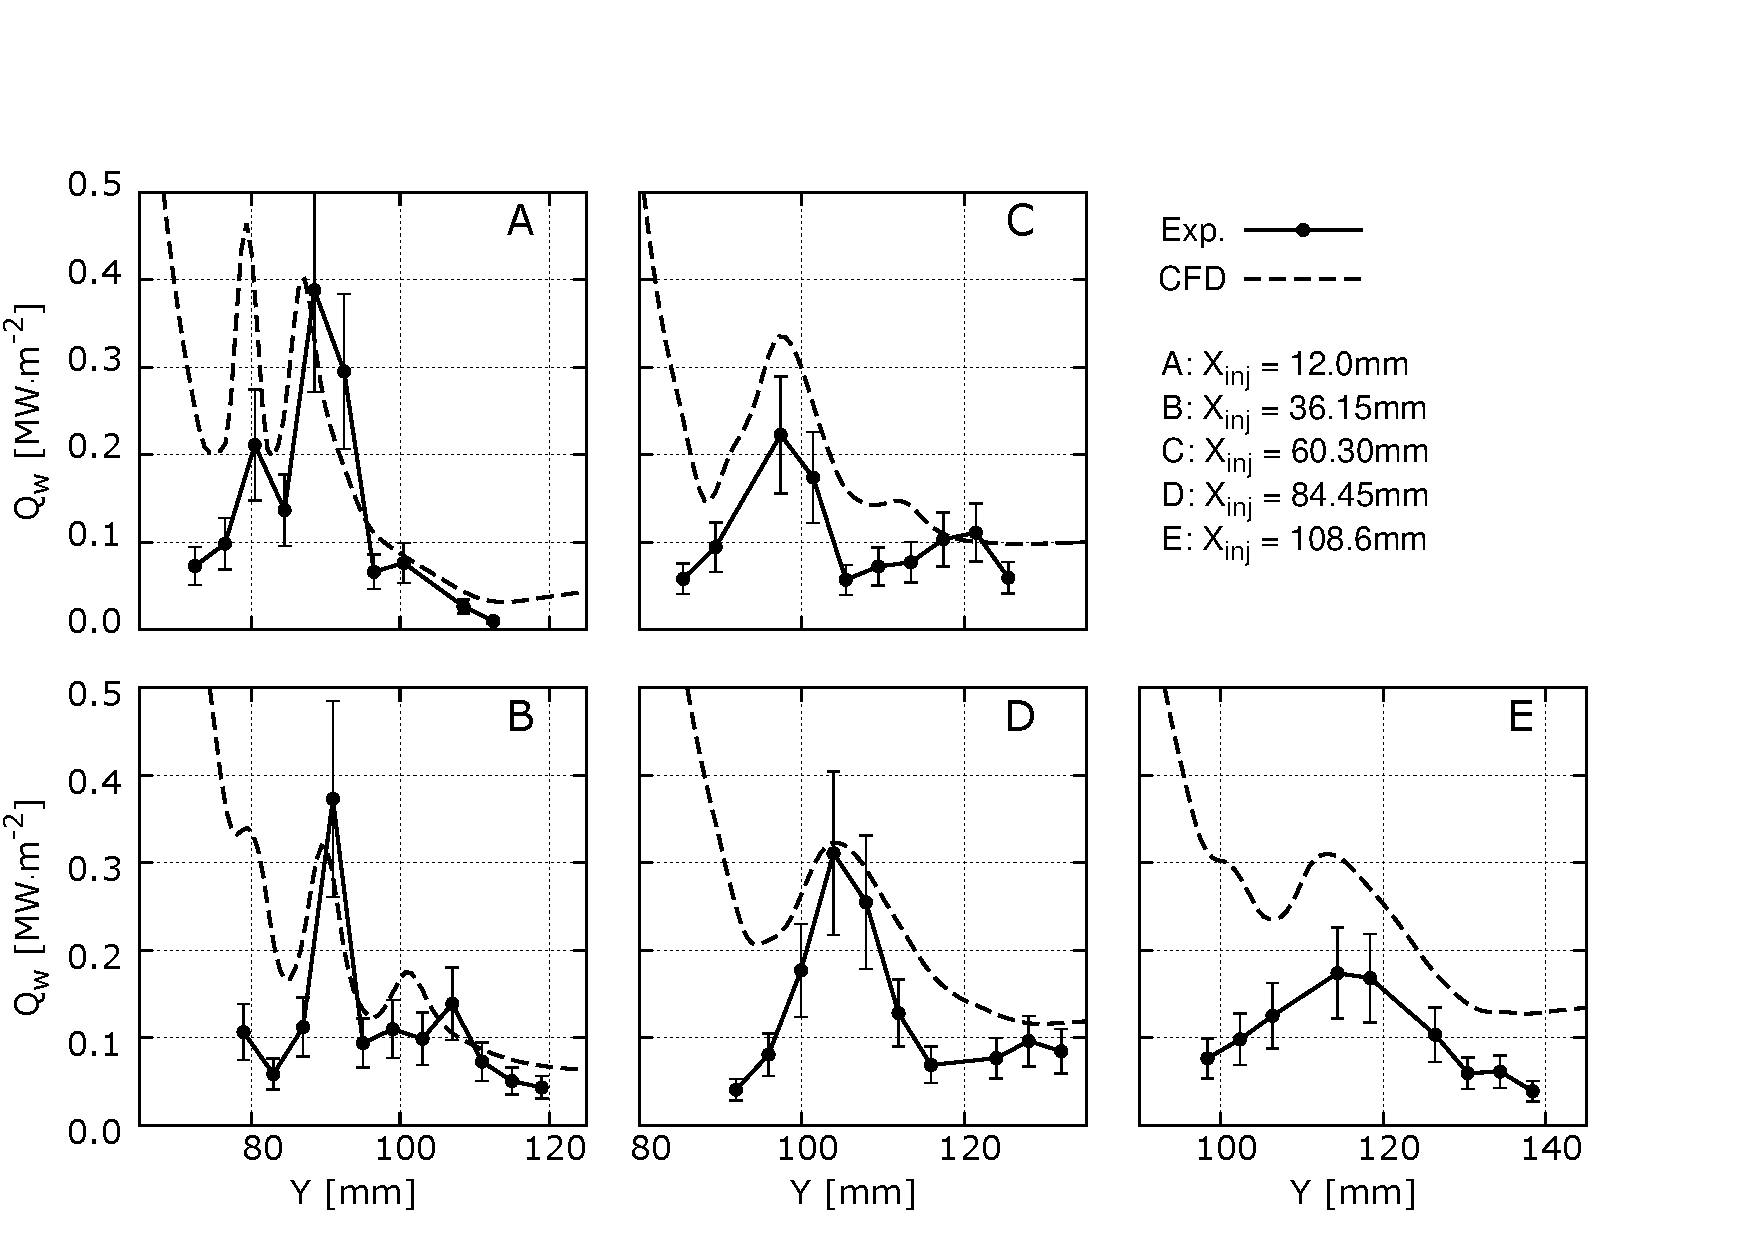
\includegraphics[trim = 0mm 3mm 25mm 25mm, clip, width=0.60\columnwidth,valign=t,fbox]{Figures/Data/LP_LI_UF/GNUP_CFD_GaugesLines_Multi.pdf}
\caption{Numerical and experimental heat transfer data. LI-UF (Case 2 in Table~\ref{tab:T4_Test_Cases})}
\label{fig:HeatFluxLPLIUF}
\end{figure} 
%

Despite the similarities between the low and high injection cases, the low injection case shows a larger discrepancy between numerical and experimental data in the `numerical overestimation zone'. 

In the high injection pressure case (HI-UF), the injection bow shock has a larger effect on heat flux, helping to mask the intrinsic error produced near the fin shock. In this case (LI-UF), the lower injection pressure makes the numerical error in the `numerical overestimation zone' more apparent. This is specially visible in lines A and E. In Line A, the left hand side peak is clearly overestimated due to its proximity to the fin shock. In Line E, the effect of the injection bow shock is substantially dissipated, incrementing the discrepancy between the lines due to effect of the `numerical overestimation zone'.

\subsubsection{Lower fin position, High injection pressure}

The heat flux results for the high injection pressure, low fin position (HI-LF) are presented in Fig.~\ref{fig:HeatFluxLPHILF}.
These lines show very good agreement across the whole domain. This case shows a better agreement between the numerical and experimental data than the case with the Upper fin position. As previously described, the fin shock in the Lower fin position is further from the data acquisition region. Thus, a smaller area of the `numerical overestimation zone' is affecting the measurements. This improvement is specially visible in Line A, where the experimental data points even for the left hand side peak lie very close to the numerical data line.
%
%LP_HI_LF
\begin{figure}[!h]
\center
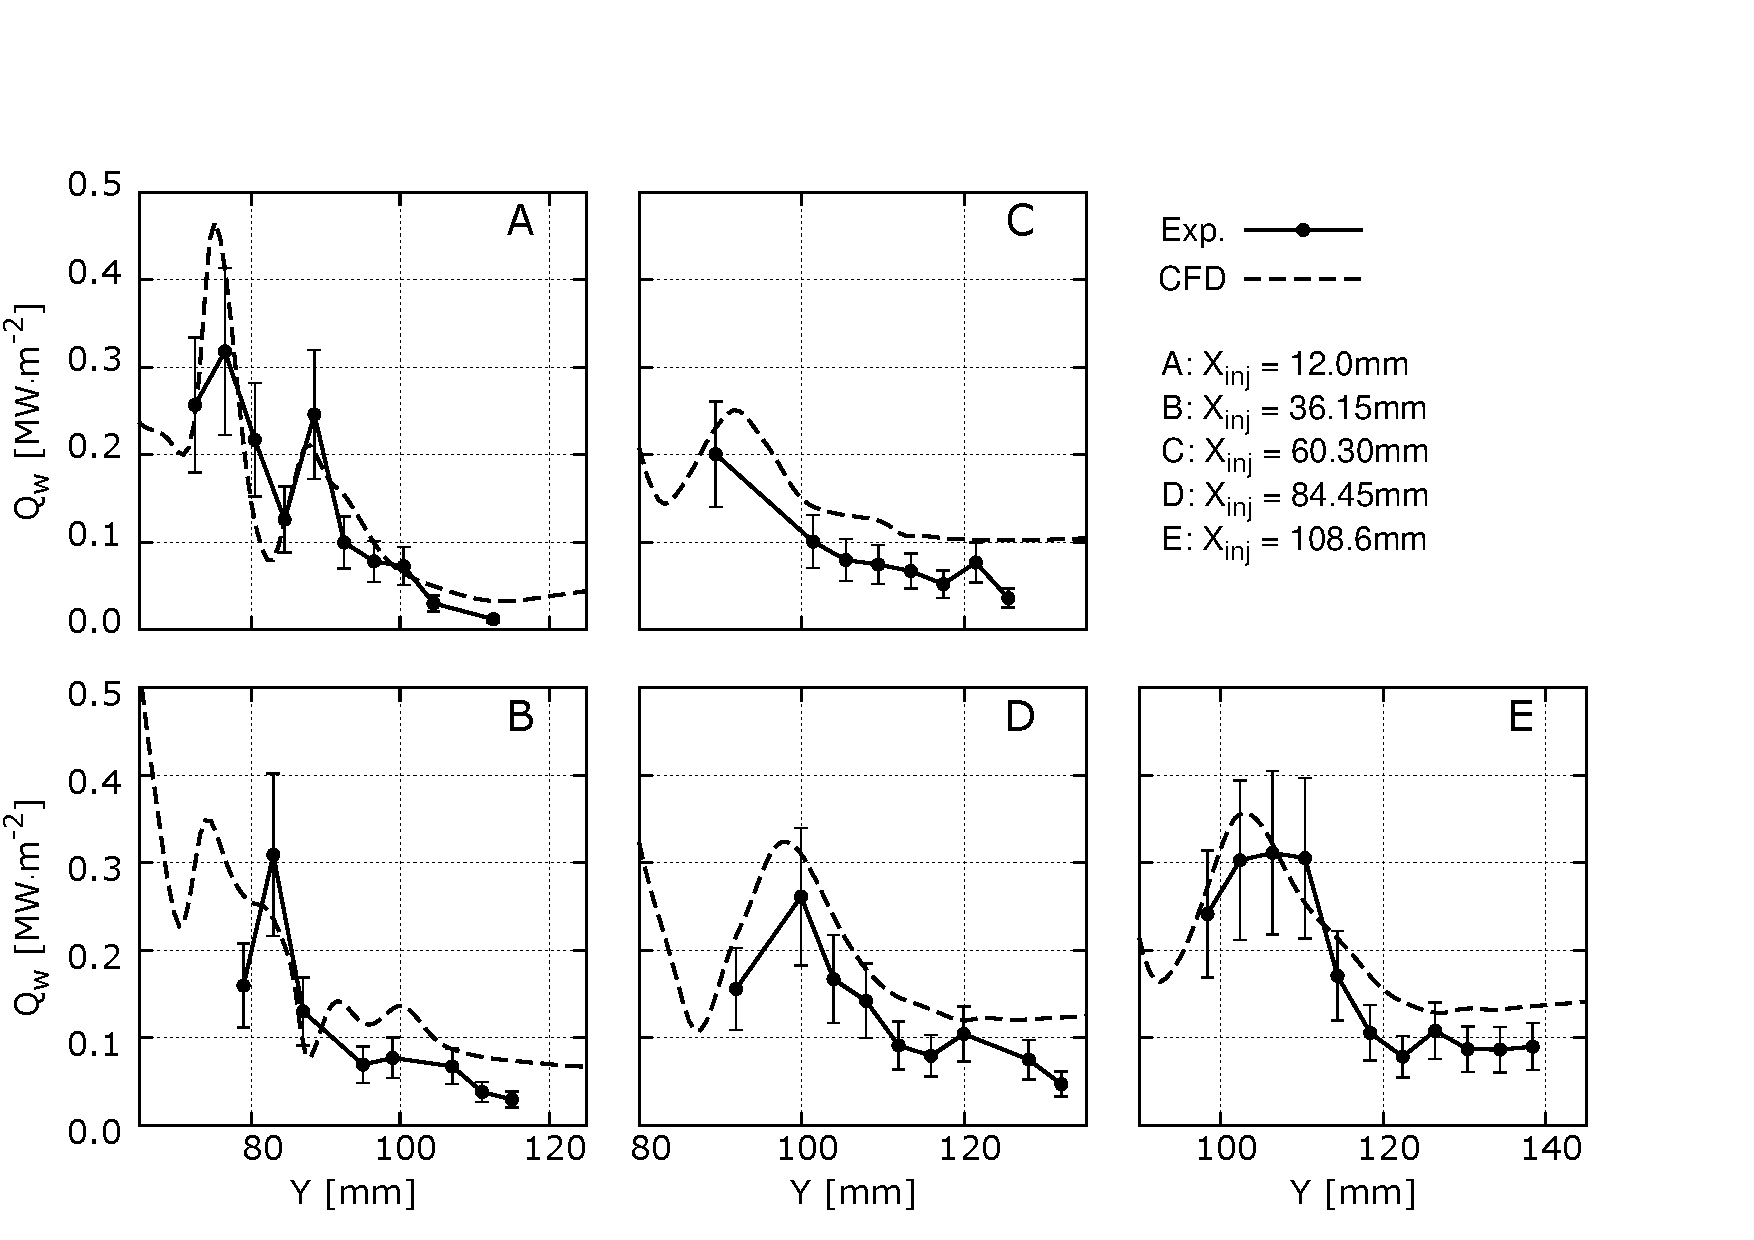
\includegraphics[trim = 0mm 3mm 25mm 25mm, clip, width=0.60\columnwidth,valign=t,fbox]{Figures/Data/LP_HI_LF/GNUP_CFD_GaugesLines_Multi.pdf}
\caption{Numerical and experimental heat transfer data. HI-LF (Case 3 in Table~\ref{tab:T4_Test_Cases})}
\label{fig:HeatFluxLPHILF}
\end{figure} 

The agreement between the numerical and experimental heat flux data is very satisfactory. Not only the location of the heat flux peaks is well captured, but also the heat flux value is accurately predicted. 

% % % % % %
% % % % % % % 
 
\subsubsection{Lower fin position, Low injection pressure}
 
The Lower fin Low injection case, low fin position heat flux data is presented in Fig.~\ref{fig:HeatFluxLPLILF}. Again, thanks to the fin shock sitting further form the measurement region, the effect of the `numerical overestimation zone' is reduced compared to the high fin position case with Low injection pressure. 
Nonetheless, the accuracy of the numerical results is slightly lower than in the equivalent case with high injection pressure. As for the Upper fin cases, this is due to the lower effect of the injection bow shock on heat flux. This makes the tendency to overestimate heat flux near the fin in the numerical results more visible. 
%
\begin{figure}[!h]
\center
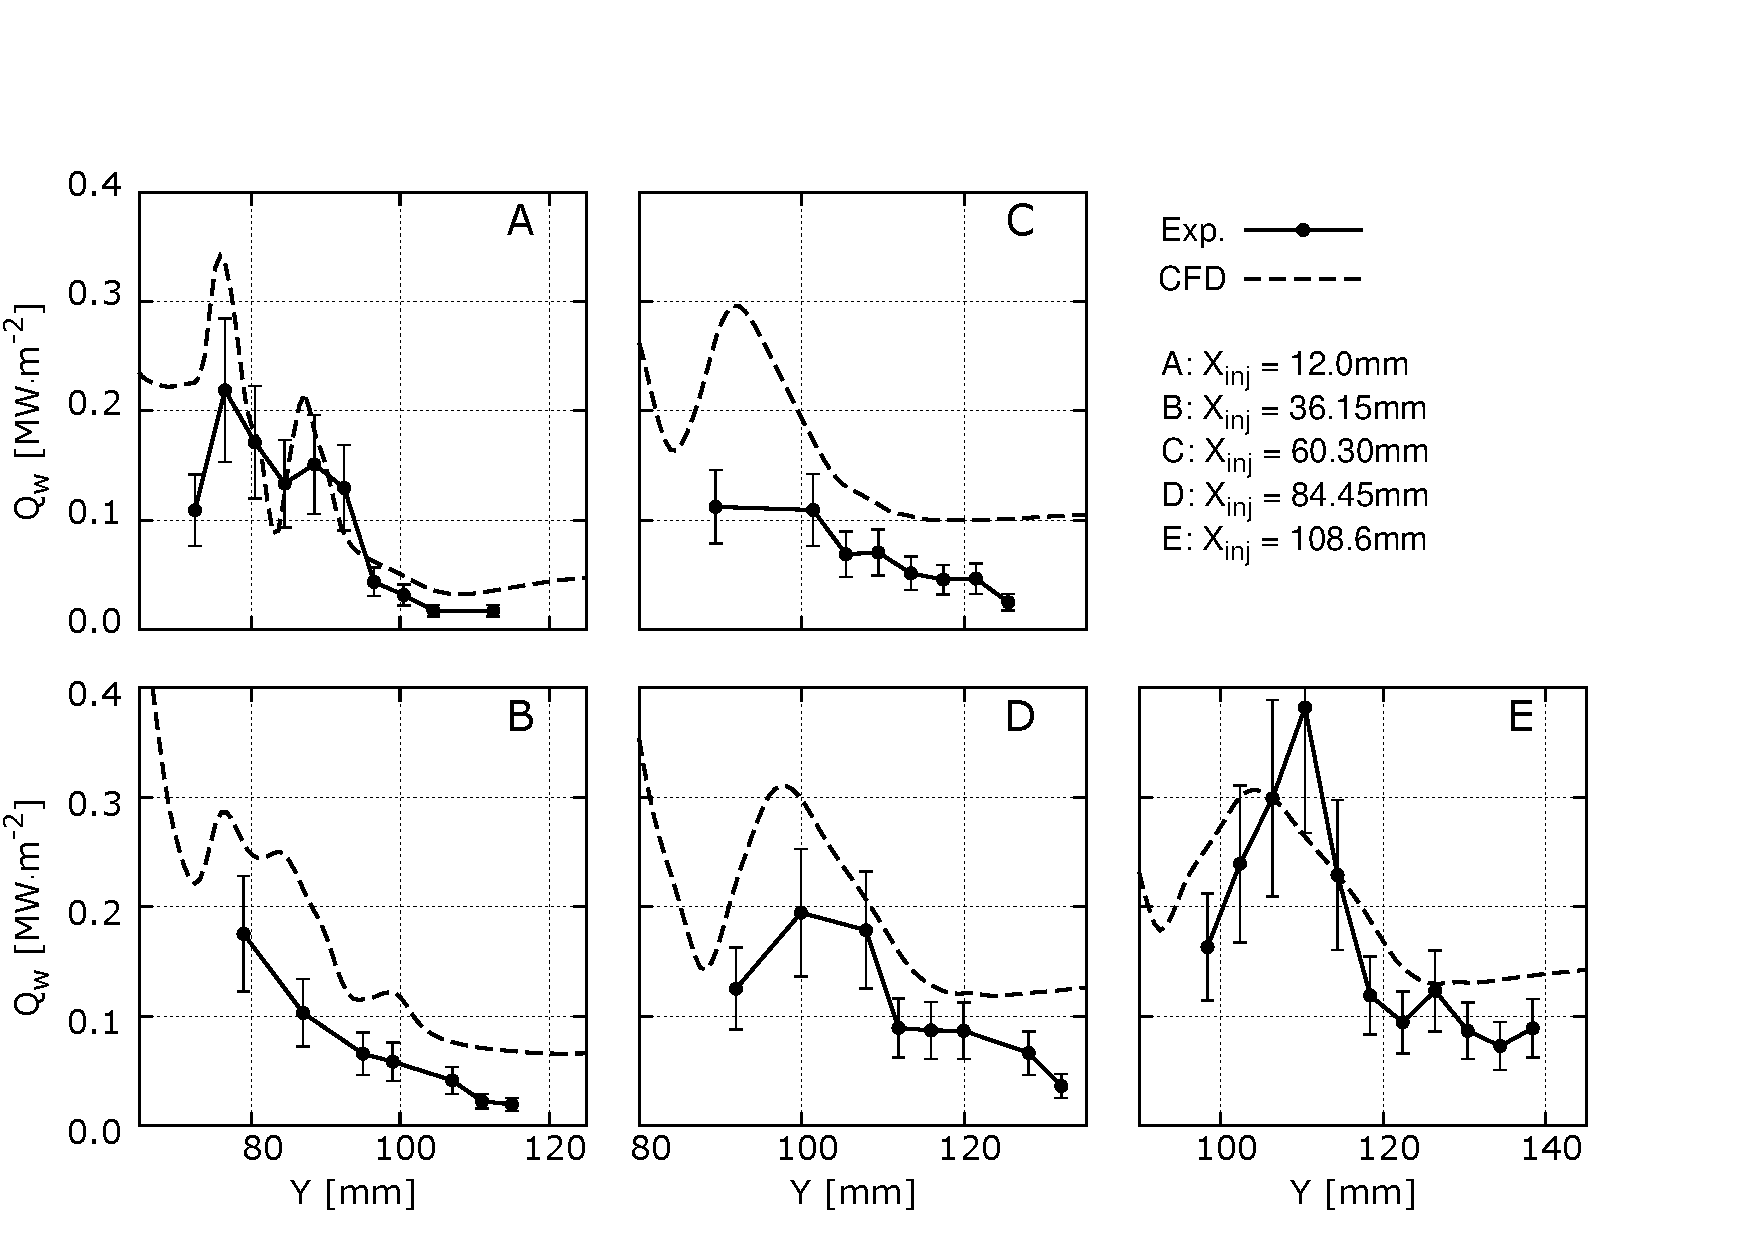
\includegraphics[trim = 0mm 3mm 25mm 25mm, clip, width=0.60\columnwidth,valign=t,fbox]{Figures/Data/LP_LI_LF/GNUP_CFD_GaugesLines_Multi.pdf}
\caption{Numerical and experimental heat transfer data. LI-LF (Case 4 in Table~\ref{tab:T4_Test_Cases})}
\label{fig:HeatFluxLPLILF}
\end{figure} 



\section{Conclusions}

A canonical geometry consisting of a flat plate plus fin with compression angle has been used to generate vortices representative of those intrinsically generated by scramjet inlets. By injecting within the vortex, the vortex-injection interaction and its effect on heat flux was studied. The data was obtained both experimentally and numerically, allowing to assess the ability of the numerical methodology to predict the experimental results.

The vortex measurements with no injection showed a localized region of severe mismatch between experimental and numerical data. This limitation of the numerical methodology was identified as a tendency to overpredict turbulent intensity by the $SST k-\omega$ turbulence model on the flat plate surface in the region adjacent to the fin shock. The effect of the overprediction near the fin shock affects the numerical data also in the vortex-injection tests. This effect was found to be less severe as the fin shock is moved away form the data acquisition region by moving the fin.

Despite the limitations of the numerical methodology due to the local overprediction heat flux, the location of the injection bow shock and secondary counter-rotating vortex were very accurately retrieved. Moreover, the heat flux levels were satisfactorily accurate in the regions not adjacent to the fin shock. This suggests the flowfield is accurately predicted in by the numerical methodology.


\section{Bibliography}

\begin{thebibliography}{}

% KDB: I'm just going to throw these in here. I'll let you organize how you want to include them. We could probably also reference their papers if you feel so inclined.

\bibitem{Wise2014b}
Wise, D. J., \& Smart, M. K. (2014). Roughness-Induced Transition of Hypervelocity Boundary Layers. Journal of Spacecraft and Rockets, 51(3), 847–854. https://doi.org/10.2514/1.A32674


\bibitem{Hunt2009}
Hunt, D. C., Paull, A., Boyce, R. R., \& Hagenmaier, M. (2009). Investigation of an Axisymmetric Scramjet Configuration Utilising Inlet Injection and Radical Farming. In 19th International Symposium on Airbreathing Engines (ISABE2009).


\bibitem{Itoh1999}
Itoh, K., Ueda, S., Komuro, T., Sato, K., Tanno, H., \& Takahashi, M. (1999). Hypervelocity aerothermodynamic and propulsion research using a high enthalpy shock tunnel HIEST. In 9th International Space Planes and Hypersonic Systems and Technologies Conference.


\bibitem{Stalker_2005}
Stalker, R. J., Paull, A., Mee, D. J., Morgan, R. G., \& Jacobs, P. A. (2005). Scramjets and shock tunnels -The Queensland experience. Progress in Aerospace Sciences, 41, 471–513.


\bibitem{RidingsAndrewNoel2015Iops}
Ridings, A. N. (2015). Investigation of pre-combustion shock trains in a scramjet using a shock tunnel at Mach 8 flight conditions. The University of Queensland, School of Mechanical and Mining Engineering.


\bibitem{Chan:Boundary_Layer_Combustion_Perturbation}
Khang, W. C. Y. (2012). Effects of flow non-uniformities on the drag reduction by boundary layer combustion, (August).


\bibitem{Doherty:PhD_Thesis_Scram_M10}
Doherty, L. J. (2013). Experimental Investigation of an Airframe Integrated 3-D Scramjet at a Mach 10 Flight Condition. University of Queensland.


\bibitem{Kirchhartz:PhD_Thesis_Boundary_Combustion}
Kirchhartz, R. M. (2009). Upstream Wall Layer Effects on Drag Reduction with Boundary Layer Combustion. University of Queensland.


\bibitem{Tanimizu:Phd_Thesis}
Tanimizu, K. (2008). Nozzle Optimization Study and Measurements for a Quasi-Axisymmetric Scramjet Model. University of Queensland.


%1
\bibitem{SmartTetlow}
Smart, M.~K. \& Tetlow, M.~R., {\it Orbital delivery of small payloads using hypersonic airbreathing propulsion}, J. Spacecraft Rockets, {\bf 46, No.1}, 2009, 117-125.
%2
\bibitem{CookHueter}
Cook, S. \& Hueter, U., {\it NASA's integrated space transportation plan 3rd generation reusable launch vehicle technology update}, Acta Astronautica, 53, 2003, 719-728.
%3
\bibitem{Alvi}
Alvi, F.~S. \& Settles, G.~S., {\it Physical model of the swept shock wave/boundary-layer interaction flowfield}, AIAA Journal, 30, No.9, 1992, 2252-2258.
%4
\bibitem{Llobet_PlumeElongation}
Llobet, J.~R., Gollan, R.~J., \& Jahn, I.~H., {\it Scramjet inlet vortices: its effect on fuel plume elongation and mixing rate}, publication pending.
%5
\bibitem{SpacePlanes_paper2015}
Llobet, J.~R., Jahn, I.~H. \& Gollan, R.~J., {\it Effect of stream-wise Vortices on Scramjets Porthole Injection Mixing}, Proceedings for the 20th AIAA International Space Planes and Hypersonic Systems and Technologies Conference, Glasgow, 2015. 
%6
\bibitem{Stalker1966}
Stalker, R~.J., {\it The Free-Pison Shock Tube}, The Aeronautical Quarterly, 1966, 351-370.
%7
\bibitem{AFMCpaper2014}
Llobet, J.~R., Barth, J.~E. \& Jahn, I.~H., {\it Vortex Tracking Algorithm for Hypersonic Flow in Scramjets}, 19th AFMC, 8-11 December, Melbourne 2014. Submitted for publication.
%8
\bibitem{JSASS_paper}
Llobet, J.~R., Jahn, I.~H. \& Gollan, R.~J., {\it Effect of vortex-injection interaction on wall heat transfer in a flat plate with fin corner geometry}, Trans. JSASS Aerospace Tech. Japan, Vol.15, No.APISAT-2016, 2017, a17-a26. 
%9
\bibitem{Wise_Thesis}
Wise, D., {\it Experimental Investigation of a 3D Scramjet Engine at Hypervelocity Conditions}, PhD thesis, The University of Queensland, 2014.
%10
\bibitem{Schultz_Book}
Schultz, D. \& Jones, T., {\it Heat-Transfer Measurements in Short-Duration Hypersonic Facilities}, AGARD-AG-165, North Atlantic Treaty Organization Advisory Group for Aerospace Research and Development, 1973.
%11
\bibitem{nenzfr_manual}
Doherty, L., Zander, F. , Jacobs, P., Gollan, R., Chan, W., \& Kirchhartz, R., {\it NENZF-r: Non-Equilibrium Nozzle Flow, Reloaded. A User Guide.}, Mechanical Engineering Report 2012/08, The University of Queensland School of Mechanical and Mining Engineering, 2012.
%12
\bibitem{Eilmer3UserGuide}
P.~A. Jacobs, \& R.~J. Gollan., {\it The Eilmer3 Code: User Guide and Example Book.}, Mechanical Engineering Report 2008/07, The University of Queensland School of Mechanical and Mining Engineering, 2009.
%13
\bibitem{Eilmer_TheoryBook}
P.~A. Jacobs, R.~J. Gollan, A.~J. Denman, B.~T. O'Flaherty, D.~F. Potter, P.~J. Petrie-Repar, \& I.~A. Johnston., {\it Eilmer's Theory Book: Basic Models for Gas Dynamics and Thermochemistry.}, Mechanical Engineering Report 2010/09, The University of Queensland School of Mechanical and Mining Engineering, 2010.
%14
\bibitem{CEA2}
McBride, B.~J., \& Gordon, S., {\it Computer program for calculation of complex chemical equilibrium	compositions and applications. Part 2: User manual and program description.}, Reference Publication 1311, NASA, 1996.


\end{thebibliography}
\end{document}
